% Options for packages loaded elsewhere
% Options for packages loaded elsewhere
\PassOptionsToPackage{unicode}{hyperref}
\PassOptionsToPackage{hyphens}{url}
\PassOptionsToPackage{dvipsnames,svgnames,x11names}{xcolor}
%
\documentclass[
  10pt,
]{article}
\usepackage{xcolor}
\usepackage{amsmath,amssymb}
\setcounter{secnumdepth}{5}
\usepackage{iftex}
\ifPDFTeX
  \usepackage[T1]{fontenc}
  \usepackage[utf8]{inputenc}
  \usepackage{textcomp} % provide euro and other symbols
\else % if luatex or xetex
  \usepackage{unicode-math} % this also loads fontspec
  \defaultfontfeatures{Scale=MatchLowercase}
  \defaultfontfeatures[\rmfamily]{Ligatures=TeX,Scale=1}
\fi
\usepackage{lmodern}
\ifPDFTeX\else
  % xetex/luatex font selection
\fi
% Use upquote if available, for straight quotes in verbatim environments
\IfFileExists{upquote.sty}{\usepackage{upquote}}{}
\IfFileExists{microtype.sty}{% use microtype if available
  \usepackage[]{microtype}
  \UseMicrotypeSet[protrusion]{basicmath} % disable protrusion for tt fonts
}{}
\makeatletter
\@ifundefined{KOMAClassName}{% if non-KOMA class
  \IfFileExists{parskip.sty}{%
    \usepackage{parskip}
  }{% else
    \setlength{\parindent}{0pt}
    \setlength{\parskip}{6pt plus 2pt minus 1pt}}
}{% if KOMA class
  \KOMAoptions{parskip=half}}
\makeatother
% Make \paragraph and \subparagraph free-standing
\makeatletter
\ifx\paragraph\undefined\else
  \let\oldparagraph\paragraph
  \renewcommand{\paragraph}{
    \@ifstar
      \xxxParagraphStar
      \xxxParagraphNoStar
  }
  \newcommand{\xxxParagraphStar}[1]{\oldparagraph*{#1}\mbox{}}
  \newcommand{\xxxParagraphNoStar}[1]{\oldparagraph{#1}\mbox{}}
\fi
\ifx\subparagraph\undefined\else
  \let\oldsubparagraph\subparagraph
  \renewcommand{\subparagraph}{
    \@ifstar
      \xxxSubParagraphStar
      \xxxSubParagraphNoStar
  }
  \newcommand{\xxxSubParagraphStar}[1]{\oldsubparagraph*{#1}\mbox{}}
  \newcommand{\xxxSubParagraphNoStar}[1]{\oldsubparagraph{#1}\mbox{}}
\fi
\makeatother


\usepackage{longtable,booktabs,array}
\usepackage{calc} % for calculating minipage widths
% Correct order of tables after \paragraph or \subparagraph
\usepackage{etoolbox}
\makeatletter
\patchcmd\longtable{\par}{\if@noskipsec\mbox{}\fi\par}{}{}
\makeatother
% Allow footnotes in longtable head/foot
\IfFileExists{footnotehyper.sty}{\usepackage{footnotehyper}}{\usepackage{footnote}}
\makesavenoteenv{longtable}
\usepackage{graphicx}
\makeatletter
\newsavebox\pandoc@box
\newcommand*\pandocbounded[1]{% scales image to fit in text height/width
  \sbox\pandoc@box{#1}%
  \Gscale@div\@tempa{\textheight}{\dimexpr\ht\pandoc@box+\dp\pandoc@box\relax}%
  \Gscale@div\@tempb{\linewidth}{\wd\pandoc@box}%
  \ifdim\@tempb\p@<\@tempa\p@\let\@tempa\@tempb\fi% select the smaller of both
  \ifdim\@tempa\p@<\p@\scalebox{\@tempa}{\usebox\pandoc@box}%
  \else\usebox{\pandoc@box}%
  \fi%
}
% Set default figure placement to htbp
\def\fps@figure{htbp}
\makeatother





\setlength{\emergencystretch}{3em} % prevent overfull lines

\providecommand{\tightlist}{%
  \setlength{\itemsep}{0pt}\setlength{\parskip}{0pt}}



 
\usepackage[backend=biber,style=numeric,sorting=none]{biblatex}
\addbibresource{references.bib}


\usepackage[margin=1in]{geometry}
\usepackage{tikz}
\usepackage{adjustbox}
\usepackage{placeins}
\usepackage{appendix}
\usepackage{amsmath}
\usepackage{subfig}
\usepackage[colorlinks = true,
            linkcolor = black,      % internal links (sections, figures, tables)
            urlcolor  = blue,       % URL links (like your latest version link)
            citecolor = black,      % citation links
            anchorcolor = black]{hyperref}
\usepackage{booktabs}
\usepackage{longtable}
\usepackage{array}
\usepackage{multirow}
\usepackage{wrapfig}
\usepackage{float}
\usepackage{colortbl}
\usepackage{pdflscape}
\usepackage{tabu}
\usepackage{threeparttable}
\usepackage{threeparttablex}
\usepackage[normalem]{ulem}
\usepackage{makecell}
\usepackage{xcolor}
\makeatletter
\@ifpackageloaded{caption}{}{\usepackage{caption}}
\AtBeginDocument{%
\ifdefined\contentsname
  \renewcommand*\contentsname{Table of contents}
\else
  \newcommand\contentsname{Table of contents}
\fi
\ifdefined\listfigurename
  \renewcommand*\listfigurename{List of Figures}
\else
  \newcommand\listfigurename{List of Figures}
\fi
\ifdefined\listtablename
  \renewcommand*\listtablename{List of Tables}
\else
  \newcommand\listtablename{List of Tables}
\fi
\ifdefined\figurename
  \renewcommand*\figurename{Figure}
\else
  \newcommand\figurename{Figure}
\fi
\ifdefined\tablename
  \renewcommand*\tablename{Table}
\else
  \newcommand\tablename{Table}
\fi
}
\@ifpackageloaded{float}{}{\usepackage{float}}
\floatstyle{ruled}
\@ifundefined{c@chapter}{\newfloat{codelisting}{h}{lop}}{\newfloat{codelisting}{h}{lop}[chapter]}
\floatname{codelisting}{Listing}
\newcommand*\listoflistings{\listof{codelisting}{List of Listings}}
\makeatother
\makeatletter
\makeatother
\makeatletter
\@ifpackageloaded{caption}{}{\usepackage{caption}}
\@ifpackageloaded{subcaption}{}{\usepackage{subcaption}}
\makeatother
\usepackage{bookmark}
\IfFileExists{xurl.sty}{\usepackage{xurl}}{} % add URL line breaks if available
\urlstyle{same}
\hypersetup{
  pdftitle={Uneven Wage Growth and Public Goods},
  pdfauthor={Ebba Mark},
  colorlinks=true,
  linkcolor={blue},
  filecolor={Maroon},
  citecolor={Blue},
  urlcolor={Blue},
  pdfcreator={LaTeX via pandoc}}


\title{Uneven Wage Growth and Public Goods}
\usepackage{etoolbox}
\makeatletter
\providecommand{\subtitle}[1]{% add subtitle to \maketitle
  \apptocmd{\@title}{\par {\large #1 \par}}{}{}
}
\makeatother
\subtitle{The Case of US Public Education}
\author{Ebba Mark}
\date{2026-01-07}
\begin{document}
\maketitle

\begin{center}
\textit{Latest version available \href{https://ebbam.github.io/pub_fin_schools/code/regressions.pdf}{here}.}
\end{center}
\begin{abstract}
 Wage growth is a key driver of local wealth accumulation, enabling greater household and community investment in public goods. Unfortunately, wage growth has diverged markedly from productivity growth in the United States in recent decades. As such, regions whose wages track productivity gains tend to benefit from broader economic growth, while lagging regions risk weaker savings capacity and declining support for public services. This work estimates the effect of local wage shocks on education spending using a shift-share instrumental variable design, exploiting variation in commuting zone industrial composition interacted with national industry growth shocks. We estimate that a 10\% increase in local wages generates a 2.3\% short-run increase in per-pupil education expenditure, with a long-run effect of approximately 4.6\%. This result is only driven by a handful of states, whereas others exhibit little wage responsiveness. These results expedite the need to enable education equalisation programmes to account for future potential wage disparities.
\end{abstract}


\section{Introduction}\label{introduction}

\textbf{Since the 1970s, the United States has experienced a persistent
divergence between productivity growth and wage growth}
\autocite{hoffmann2020,stansbury,economicpolicyinstitute,elsby2013}.
While labor productivity has continued to rise, the earnings of typical
workers have increased far more slowly, leading to a substantial
decoupling between the two trends. Explanations range from heterogeneous
demand for human capital
\autocite{autor2014,katz1992,acemoglu2012,autor2011,autor_growth_2013}
to competition \autocite{stansbury,deb2022,yeh2022,azar2022,wilmers2018}
to weakened labor market institutions and policy forces
\autocite{egger2019,lee1999,mishel2021,barkai2020,autor2016,card2001,bivens2013,stansbury2020}.\footnote{Summers
  \& Stansbury 2018 argue that productivity growth still exerts a
  positive influence on wages overall, but that institutional and
  structural changes have weakened the link for large segments of the
  workforce \autocite{summers2018,stansbury}. They point to declining
  union density, erosion of the minimum wage, globalization, and
  increased market concentration as key factors that have shifted
  bargaining power away from workers and reduced labor's share of
  national income \autocite{autor2014}. Furthermore, additional evidence
  finds that this decoupling is far from a universal phenomenon. Rather,
  decoupling applies almost strictly to lower- and medium-wage earners,
  while already higher wages manage to keep up (relatively) with
  productivity growth rates.} Though its causes are hotly debated, the
fact itself is well-documented, especially for lower- and middle-income
workers \autocite{komlos2018}.\footnote{Though authors find that wage
  inequality growth has stagnated in the last decade, this is not a
  result of a ``catch-up'' effect of lower- or middle-income earners
  with top income earners, but rather wage growth at the bottom of the
  wage distribution \autocite{aeppli2022}. Additionally, further
  evidence indicates that metric choice can influence the ambiguity of
  earnings and wage inequality conclusions \autocite{parolin2025}.}

\textbf{Regardless of its causes, the decline in the wage–productivity link has important consequences.}
Wages remain the most direct channel through which national productivity
growth translates into household well-being. When wage growth lags
productivity, improvements in aggregate efficiency do not translate into
broad-based improvements in living standards \autocite{mishel2021}.
Furthermore, in a context in which the benefits of economic growth have
already accrued unevenly across communities in the United States, this
pattern may reinforce existing spatial inequalities in economic
activities, especially in regions where industrial composition and
historical shocks have already left communities economically vulnerable
\autocite{bauluz,rickard2020,fee2025,storper2009,fallah2011,benmelech,greenstone2010}.

\textbf{A link that has been far less explored in this context is the
spillover effect of local wages to local wealth-building and its effect
on public goods.} Wage growth is an important contributor to local
wealth-building, allowing households and communities to invest more in
local public goods \autocite{boustan2013}. Communities whose wages rise
in line with productivity growth will likely reap the benefits of
economic growth whereas those who do not, risk falling behind. This link
is particularly important in the US given the structure of local public
financing. Majority of local public services are funded via property
taxes. This funding structure entrenches a mechanism for generating
inequality of opportunity between diversely affluent regions of the
country
\autocite{manduca2025,weir2021,schechtl2024,mettler2011}.\footnote{A
  burgeoning literature points to the role of racial segregation and its
  enduring legacy in perpetuating inequality in local economic health,
  wealth, and public service expenditure
  \autocite{avenancio-león2022,trounstine2016,trounstine2021}.} Existing
work shows that income inequality and uneven local income growth shape
inequalities in local public goods provision, residential mobility, and
long-run opportunity \autocite{chetty2014}. Wage stagnation can
translate directly into weakened fiscal capacity. Put plainly, given the
structure of US public services, wherein they are tied to asset values,
inequality in wealth-building can have significant effects for the
quality of local public services.

\textbf{Community well-being and public expenditure in the US is already
characterized by a high degree of spatial heterogeneity
\autocite{manduca2025,obrien2025,feler2017,chetty2026}.} Evidence of how
income inequality perpetuates other forms of inequality (opportunity,
health, infrastructure quality, and broader well-being) is steadily
increasing
\autocite{chetty2016,logan2012,semuels2016,Avancena2021,flavin2009,boustanEffectRisingIncome2013}
find that greater income inequality leads to higher public expenditure
across all public goods indicating that a presence of higher-earners in
a local area contributes to higher levels of expenditure. Though this
does not support an unambiguous denunciation of inequality in itself, it
provides additional evidence for the fact that local incomes affect
public expenditure raising the potential for ``superstar'' and ``left
behind'' regions to emerge absent even income growth.

\textbf{Local public education is particularly relevant in this
context.} Public schools are responsible for education over 80\% of
American school-age children. In 2019, governments around the US
(including the federal government) spent a total of \$870 billion on
public education, roughly \$17,013 per pupil
\autocite{nationalcenterforeducationstatistics2023,skinner2019}.
However, the quality of services delivered and fiscal resources spent
vary widely across the country \autocite{biolsi2022}. A sometimes
lacking, or at best under-performing, federal equalization system
perpetuates this structural force
\autocite{beland2017,biasi2023,hoxby1998,mccabe2019,baker2016,aesa2024}.
Take Connecticut for example. In 2016, according to the Connecticut
State Department of Education, the town of Greenwich town, one of the
highest-income towns in the country, spent \$22,000 per pupil while
Bridgeport, although only located 40 kilometers away, spent \$14,000
\autocite{semuels2016}.

\textbf{The quality of public education, especially at an early age, can
have long-lasting consequences for personal and economic well-being over
an individual's lifetime as well as generations following them}
\autocite{alfonso2020,zheng2022}. Although only a small piece of the
puzzle that determines quality public education, expenditure levels
ensure adequate funding for facilities, teachers, administrators, and
other services \autocite{baker2017,baker2025,jackson2016}. Furthermore,
evidence suggests that progressive spending delivers efficiency gains in
school performance \autocite{rauscher2022}. Therefore, ensuring that
local or regional economic decline does not disrupt or worsen the
quality of education delivered is of paramount importance to ensure
greater equality in the long-run. Altogether, this evidence points to
the value of identifying the extent to which expenditure on public
education is reliant on local wage growth across the country.

\textbf{Despite the large literature on the existence of
wage-productivity decoupling, inequality in local public goods
provision, and US school financing system, one central link remains
under-explored: Are local public education budgets sensitive to local
wages, and if so, for whom and under what conditions?}

To be more precise, this study investigates the following questions:

\emph{RQ1:} Do local wage gains affect public education expenditure in
levels?

\emph{RQ2:} If so, is this relationship constant across commuting zones?
What sources of heterogeneity mediate this relationship?

\emph{RQ3:} In light of recent reforms to intergovernmental education
funding aimed at reducing disparities in educational expenditure, do
intergovernmental transfers mitigate wealth-driven inequalities in
public education spending?

\subsection{Theoretical Motivation and Empirical
Approach}\label{theoretical-motivation-and-empirical-approach}

Although as mentioned above, existing work provides descriptive evidence
that higher income communities invest more in local services, the causal
effect of wage growth on education spending is unclear due to
substantial endogeneity. Any study of the linkage between two or more
local socio-economic outcomes presents considerable endogeneity
challenges. Higher-wage households select into districts with better
schools. Education quality affects local human capital and, thus, wages.
Local fiscal decisions respond to political, demographic, and
institutional environments that co-evolve with economic conditions.
Moreover, regional heterogeneity is large. States differ in their
reliance on local versus state funding; commuting zones differ in
industrial composition and exposure to national shocks; and localities
vary in their ability to translate tax bases into expenditures. On a
cultural level, the quality of local education can potentially impact
preferences for education in turn. Thus, a national ``average'\,'
elasticity may be misleading. What is missing is a causally identified,
regionally sensitive, and mechanism-informed estimate of the elasticity
of public education expenditure to local wages.

To overcome these challenges, we construct a shift--share instrumental
variable for local wages. More precisely, to interrogate the elasticity
of public education expenditure to wages across US commuting zones, we
construct a shift-share instrument that combines fixed local industry
employment shares with national industry-level changes in real value
added using data from the US Bureau of Labor Statistics and Bureau of
Economic Analysis. This instrument generates plausibly exogenous local
variation by exploiting how different regions are differentially exposed
to common national trends, while abstracting from endogenous local
dynamics. It is particularly well suited in this setting, since the
local tax base, and thus education spending, likely depends on
industries that are unevenly distributed across regions but subject to
similar industry-specific wage shocks. We use this instrument to
identify the effect of wage shocks on local public education expenditure
as reported by the US Census Bureau's Annual Survey of State and Local
Government Finances.

Given the substantial heterogeneity across U.S. states arising both from
structural sources (such as differences in tax systems, regulatory
environments, and legislative institutions) and from evolved
characteristics (including industrial composition, income levels,
inequality, and broader measures of economic diversity) the scope for
identifying a policy-relevant single national average treatment effect
is inherently limited. Therefore, we proceed in two steps. First, we
provide an initial benchmark using a pooled estimation to establish a
baseline relationship between wages and education expenditure that
generalizes reasonably across the national economy. Second, we
investigate the regional and industrial heterogeneity that these pooled
estimates mask via a state-by-state estimation, industry-by-industry
estimation, and grouping commuting zones by their historic wage and GDP
growth trajectories to improve comparability of treatment and control
groups in our instrumental variable design. In the latter heterogeneity
analysis, we construct commuting zone growth rates as idiosyncratic
variables absent state and national-level growth rates, understanding
that \emph{relative} growth rates are of particular importance in a
landscape where local economies determine the actual \emph{value} of
wage levels. This allows us to identify where the wage--expenditure link
is strongest or weakest.

\subsection{Main Results and
Contribution}\label{main-results-and-contribution}

\begin{enumerate}
\def\labelenumi{\arabic{enumi}.}
\item
  First, we find that public education expenditure responds strongly and
  positively to local wage growth. A 10\% increase in local wages is
  associated with a 2.2\% increase in public elementary education
  expenditure, with a long-run increase of 4.6\%.
\item
  Second, estimating the instrumental variable model separately for each
  state reveals substantial heterogeneity in the relationship between
  wages and education expenditure. Only a third of the 40 states
  analysed in this study show persistent causal relationships between
  wages and education expenditure, indicating that these carry the
  weight of national-level identification. Many of these states rely on
  an above-average share of education funding coming from local sources
  rather than intergovernmental transfers. Across these states the wage
  elasticity varies between 2-10\% increases in response to a 10\%
  increase in local wages, with Colorado, Florida, and South Dakota
  exhibiting highest wage elasticities.
\item
  Third, elasticities are largest, both in terms of size and statistical
  significance, in commuting zones with historically low wage growth
  compared to other regions, and smallest in regions with historically
  strong wage trajectories. This indicates that regions already
  experiencing economic stagnation may face compounded disadvantages
  through weaker fiscal capacity for education spending.
\end{enumerate}

As such, these results make three important contributions to the
existing literature. First, the paper provides causal estimates of the
elasticity of local public education expenditure to local wage growth
across US commuting zones, documenting both the average national
relationship and substantial regional heterogeneity.

Second, the results show that local fiscal capacity is closely tied to
historically uneven wage growth, implying that wage-productivity
decoupling has important implications not only for households but also
for public sector institutions that shape long-run opportunity. Lastly,
the paper demonstrates how the structure of the US school financing
system amplifies or dampens the effects of local economic change, with
weaker equalizing opportunities exacerbating the consequences of wage
stagnation. Together, these findings show that the wage-productivity
nexus has implications that go far beyond household earnings: it shapes
the fiscal foundations of local public education and, through that
channel, the intergenerational transmission of economic opportunity.

In the sections that follow, we outline the various data sources used in
Section~\ref{sec-data}; provide a detailed overview of our shift-share
construction and methodological approach Section~\ref{sec-methods} with
accompanying results; and conclude with a discussion of policy
implications in Section~\ref{sec-conclusion}.

\section{Data}\label{sec-data}

We compile a panel dataset of the following indicators across 636
commuting zones (CZ) in 40 US states annually between 2001-2021.

\textbf{Expenditure and Revenue:} This work relies on a harmonized
repository from Willamette University of the data collected annually as
part of the US Census Bureau's Annual Survey of State \& Local
Government Finances (SLGF). The SLGF is the `only comprehensive source
of information on the finances of local governments in the United
States' \autocite{pierson}. The data includes county-level revenue,
property taxes, and expenditure on public education including
disaggregated values by revenue source (federal, state, or other
intergovernmental revenue) and expenditure item (lunches, wages, debt).
All values are reported in real US dollars. We aggregate school district
measures up to the commuting zone-level to ensure the availability of
adequate control and treatment variables. We choose to conduct the
analysis on the commuting zone level because it is a more accurate
picture of a local labor market area
\autocite{carpenterWhenUseCommuting2022}.\footnote{The database is
  provided for six different levels of government: state, county,
  municipal, township, special district, and school district. Reporting
  is only mandated in Census years (every five years), and even then
  missing data remains a challenge. This means that data provided at any
  other level of government suffers from significant levels of missing
  data, with a high level of selection bias correlated with
  administrative capacity. However, strengthened by a partnership with
  the National Center for Education Statistics, observations for US
  school districts exhibit near-complete coverage between 1997-2021
  (\textcite{pierson}).} Our main outcome variable is per pupil spending
on elementary education.

\textbf{Population controls:} We source commuting-zone level population
statistics by aggregating data from county-level populations statistics
from the US Census Bureau

\textbf{Local GDP:} We gather local GDP control variables by aggregating
county-level GDP data from the Bureau of Economic Analysis (BEA). This
BEA data is only available after 2001, defining the lower limit of our
panel's time dimension. We primarily rely on private industry GDP as a
control variable given a large remaining portion of GDP is government
expenditure which includes public education expenditure.

\textbf{Property Prices:} The US Federal Housing Finance Agency
maintains an annual county-level Housing Price Index (HPI) metric, a
geographically linked measure of the movement of single-family house
prices. The HPI is a weighted, repeat-sales index, measuring average
price changes in repeat sales or refinancings on the same properties.
This information is obtained by reviewing repeat mortgage transactions
on single-family properties whose mortgages have been purchased or
securitized by Fannie Mae or Freddie Mac (two US government-sponsored
enterprises that guarantee most US mortgages)
\autocite{usfederalhousingfinanceagency}. We aggregate to the commuting
zone level via a population-weighted mean.

\textbf{Race Controls:} The National Institute of Health National Cancer
Institute's Surveillance, Epidemiology, and End Results (SEER) Program
provides annual estimates of total White, Black, American Indian/Alaska
Native, Asian/Pacific Islander populations at the county level,
optionally by Hispanic or non-Hispanic origin
\autocite{nationalcancerinstitutedccpssurveillanceresearchprogram}.
Though the US Census Bureau provides county-level estimates of racial
make-up of local areas in the American Community Survey, this data is
unavailable prior to 2009 and is considered less accurate than those
provided by the National Cancer Institute's SEER Database.

\textbf{Adequate Education Spending}: The University of Wisconsin's
School Finance Indicators Database provides provides detailed data on
School Funding Adequacy, measured as the dollar estimate needed per
pupil to achieve U.S. average test scores \autocite{baker}.

This data aggregation results in a complete and balanced panel of 636 US
commuting zones across 40 states between 2001-2021. \footnote{20\% of US
  states are missing from the dataset because (1) we impose an exclusion
  restriction wherein any commuting zone reporting more than five \$0
  values for property taxes collected is excluded due to likely
  measurement error and (2) Connecticut, Maryland, North Carolina, and
  Virginia have been excluded due to unconventional or incomplete public
  school district reporting.} All data used is reported annually at the
commuting zone level. \footnote{In line with similar work on US economic
  geography, commuting zones were chosen as the unit of analysis as they
  are a far less arbitrary and more accurate representation of local
  labor market areas/economies \autocite{dorn,fowler2024}.} Therefore,
apart from an indicator of a commuting zone's state, all variables are
time-variant.

\autoref{tbl_desc_stats} reports summary statistics across relevant
variables. All (dollar) values are reported in (real 2017-chained)
thousands except for the House Price Index.
\autoref{tab:tbl_order_of_integration} represents the order of
integration of relevant variables calculated using a unit root test
designed for heterogeneous panels \autocite{im2003}. All variables are
integrated I(0) indicating minimal concern for non-stationarity except
in the case of enrollment and population numbers.

\begin{table}[!htbp] \centering 
  \caption{} 
  \label{tbl_desc_stats} 
\begin{tabular}{@{\extracolsep{5pt}}lccccc} 
\\[-1.8ex]\hline 
\hline \\[-1.8ex] 
Statistic & \multicolumn{1}{c}{N} & \multicolumn{1}{c}{Mean} & \multicolumn{1}{c}{St. Dev.} & \multicolumn{1}{c}{Min} & \multicolumn{1}{c}{Max} \\ 
\hline \\[-1.8ex] 
Enrollment & 13,356 & 62.39 & 169.90 & 0.13 & 3,169.73 \\ 
Population & 13,356 & 405.18 & 1,077.99 & 0.88 & 18,732.54 \\ 
Elementary Expenditure per pupil & 13,356 & 11.39 & 2.99 & 5.97 & 58.35 \\ 
Property Tax per pupil & 13,356 & 3.60 & 2.43 & 0.29 & 32.91 \\ 
Intergovernmental (IG) Revenue per pupil & 13,356 & 7.12 & 2.28 & 1.04 & 27.50 \\ 
State IG Revenue per pupil & 13,356 & 6.73 & 2.03 & 0.79 & 26.23 \\ 
GDP per capita & 13,356 & 44.52 & 25.27 & 15.32 & 388.73 \\ 
GDP pc - Private Industry & 13,356 & 38.42 & 25.18 & 5.85 & 383.06 \\ 
House Price Index & 12,717 & 255.18 & 155.71 & 85.53 & 1,947.97 \\ 
% Black & 13,356 & 0.08 & 0.12 & 0.0005 & 0.72 \\ 
% White & 13,356 & 0.87 & 0.14 & 0.09 & 1.00 \\ 
% Hispanic & 13,356 & 0.10 & 0.15 & 0.002 & 0.96 \\ 
\hline \\[-1.8ex] 
\end{tabular} 
\end{table} 
\begin{table}
\centering
\caption{\label{tab:tbl_order_of_integration}Order of Integration}
\centering
\begin{threeparttable}
\begin{tabular}[t]{lccc}
\toprule
Variable & Order of Integration & I(0) test p-value & I(1) test p-value\\
\midrule
Enrollment & I(1) & 0.608 & <0.0001\\
Population & I(1) & 0.286 & <0.0001\\
Elementary Expenditure per pupil & I(0) & <0.0001 & \\
Property Tax per pupil & I(0) & <0.0001 & \\
Intergovernmental (IG) Revenue per pupil & I(0) & <0.0001 & \\
\addlinespace
State IG Revenue per pupil & I(0) & <0.0001 & \\
GDP per capita & I(0) & <0.0001 & \\
GDP pc - Private Industry & I(0) & <0.0001 & \\
\bottomrule
\end{tabular}
\begin{tablenotes}[para]
\item \textit{Note: } 
\item Order of integration determined using the Im-Pesaran-Shin (IPS) panel unit root test with intercept. Lag length selected via AIC with maximum of 4 lags. The null hypothesis is non-stationarity; rejection at the 5\% level indicates stationarity. I(0) denotes stationarity in levels and I(1) denotes stationarity in first differences. All variables are log-transformed prior to testing to account for heteroskedasticity.
\end{tablenotes}
\end{threeparttable}
\end{table}

Figure 1 demonstrates the spread of elementary education expenditure per
pupil by commuting zone, grouped by state. Each state's
population-weighted mean expenditure per pupil is represented in black.
There is considerable within-state variation in per-pupil expenditure
levels. Notably, Texas, Montana, and Idaho have commuting zones that
spend nearly twice as much as other zones in the same state.
Furthermore, the mean level of expenditure is nearly four times as high
in the highest-spending state (New York) than in the lowest-spending
state, Idaho. We additionally display these values in relation to the
estimated ``adequate'' level of expenditure required for students to
achieve U.S. average test scores, represented by the green and red
arrows. Majority of states fall short of the deemed adequate expenditure
value. Mississippi boasts the greatest shortfall in spending while
Wyoming boasts the greatest overshoot in spending. Figure 1 demonstrates
the considerable within state variability in spending rates as well as
between state variation in levels and student needs.

\begin{figure}[H]

{\centering \pandocbounded{\includegraphics[keepaspectratio]{regressions_files/figure-pdf/unnamed-chunk-7-1.png}}

}

\caption{Per Pupil Education Expenditure}

\end{figure}%

Figure 2 demonstrates the trajectories of local wages from an initial
level in 2001, demonstrating, the diverging wage growth trajectories of
commuting zones in our sample. Blue commuting zones represents those
exhibiting relatively high wage growth trajectories as deemed by the
calculation in Section~\ref{sec-growthrates}. The black dashed line
represents the annual national wage growth rate.

\begin{figure}

\centering{

\pandocbounded{\includegraphics[keepaspectratio]{../output/wage_trends_plot.png}}

}

\caption{\label{fig-wages}Wages and Productivity}

\end{figure}%

\section{Methods}\label{sec-methods}

\subsection{Identification Strategy}\label{identification-strategy}

We are centrally interested in the effect of changes in local wages on
public education expenditure where there is an evident endogeneity
concern between public education expenditure and wage. First, there is a
likely attracting factor of high levels of education expenditure for
higher-income families. Second, absent migration, education systems
provision local labor markets with individuals with diverse human
capital.

\begin{figure}[H]
\centering
\caption{Instrumental Variable Path Diagram}
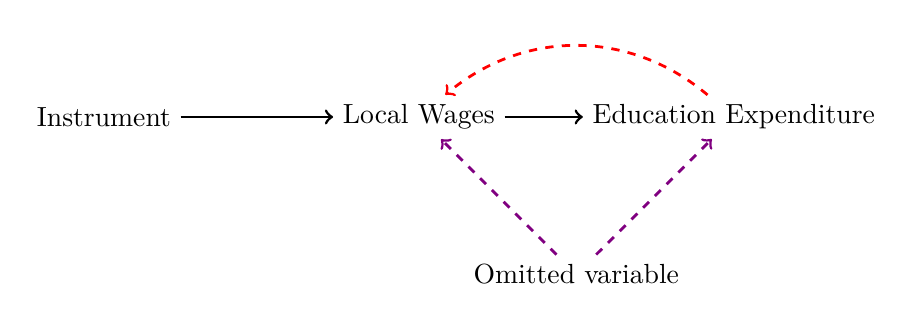
\begin{tikzpicture}
% nodes %
\node[rectangle] (z) at (0,0) {Instrument};
\node (t) at (4,0) {Local Wages};
\node (y) at (8,0) {Education Expenditure};
\node (u) at (6,-2) {Omitted variable};

% edges %
\draw[->, line width=1] (z) -- (t);
\draw[->, line width=1] (t) -- (y);
\draw[->, line width=1, violet, dashed] (u) -- (t);
\draw[->, line width=1, violet, dashed] (u) -- (y);
\draw[->, line width=1, red, bend right=40, dashed] (y) to (t);
\end{tikzpicture}
\label{fig:iv-approach}
\end{figure}

\subsubsection{Shift-share Instrument}\label{shift-share-instrument}

Therefore, we adopt a causal identification strategy via a shift-share
instrument. Shift-share or \emph{Bartik} instruments have gained
popularity in empirical work as a method of handling endogeneity issues
in panel data
\autocite{ferri2022,goldsmith-pinkham2020,bartik1991}.\footnote{Autor et
  al.~use a shift-share instrument to assess the effect of Chinese
  import competition on manufacturing employment in US commuting zones
  \autocite{autor2013}. As an extension, \autocite{feler2017} use a
  similar shift-share instrument to assess the effect of the same shock
  on the size of local government. \autocite{baccini2021} employ a
  shift-share instrument for manufacturing layoffs to tease out the
  effect of a decline in manufacturing on both economically motivated
  and racial identity voting patterns in the US.} Such instruments
combine time-variant, unit-invariant changes in aggregate economic
variables (i.e., national changes in industry value added levels) with
time-invariant, unit-variant shares in exposure to these macro-level
changes (i.e., local shares of employment in particular industries).
This decomposition of local-level changes delocalizes variation over
space and time. In doing so, it provides a defensible strategy for
`de-endogenizing' the treatment, as local exposure is predetermined with
respect to contemporaneous shocks. Moreover, by construction, the
approach enables the examination of how macro-level phenomena propagate
to and affect local units, as it generates local shocks that are driven
by national industry trends weighted but the community exposure to this
industries.\footnote{An additional popular indicator for modelling
  industrial shocks exogenously is \emph{oil price} as these values are
  often assumed to be exogenous to local and even national conditions
  \autocite{scheer2022}. Furthermore, various indicators for measuring
  \emph{deindustrialization} have been proposed including the
  manufacturing share of employment, value added, and GDP
  \autocite{tregenna2009,tregenna2020}. Finally, in rare instances,
  exogeneity can be secured due to \emph{geographical, climatological,
  or geological factors}. For example, \autocite{borge2015} obtain an
  exogenous measure of local revenue by ``instrumenting the variation in
  hydropower revenue, and thus total revenue, by topology, average
  precipitation and meters of river in steep terrain.'' Certain authors
  have argued that the fact that the location of hydrocarbon deposits is
  dictated by geomorphological processes provides a plausible argument
  for exogeneity \autocite{esposito2021,chen2022}.}

In the context of this work, we construct the instrument by interacting
commuting-zone level industrial employment shares held constant at a
base period with national real value added growth by industry. The
literature on Bartik instruments allows for an argument of plausible
exogeneity via various channels. First, authors argue that local
industry shares are exogenous by imposing that shares be fixed to a
particular base year and are therefore unable to adapt to changes in
national-level growth rates. Such a shift-share instrument is designed
as in Equation~\ref{eq-ref-bartik}.

\begin{equation}\phantomsection\label{eq-ref-bartik}{
Z_{it} = \sum_{j=1}^{k} S_{ij\tau}G_{njt}
}\end{equation}

where \(S_{ij\tau}\) is the local share of unit \(i\)'s economy
(measured using metrics like employment, wages, revenue) in industry
\(j\) at a fixed base year \(\tau\) and \(G_{njt}\) is the growth rate
of industry \(j\) at a national level \(n\) at time \(t\).

Alternatively, authors may argue that the claim of exogeneity in the
national-level growth rates is unlikely to be violated even when
allowing the local shares to vary over time. This approach is likely to
come at significant expense to instrument exogeneity. It is constructed
as follows:

\[
Z_{it} = \sum_{j=1}^{k} S_{ijt}G_{njt}
\]

Finally, authors might be concerned about the implausible exogeneity of
both shares and national-level growth rates in which case they construct
the instrument as in Equation~\ref{eq-ref-bartik-2} where the local
shares are fixed at a common base year and industry-specific growth
rates \(G\) are derived from data on other similar regions \(o\) rather
than national-level changes that are inherently comprised of local-level
shifts. This approach likely comes at significant expense to instrument
relevance.

\begin{equation}\phantomsection\label{eq-ref-bartik-2}{
Z_{it} = \sum_{j=1}^{k} S_{0jt}G_{ojt}
}\end{equation}

Finally, the authors can make an additional design choice about whether
the effect of these instruments should be assumed common to an aggregate
local-level wage growth indicator or allowed to vary by industry. In
other words, whether to construct the first-stage relationship of the
2SLS as\ldots:

\[
X_{it} = \alpha_i + \beta\sum_{j=1}^{k}S_{ijt}G_{njt} + \epsilon_{it}
\]

\ldots or\ldots:

\[
X_{it} = \alpha_i + \sum_{j=1}^{k}\beta_{j}S_{j}G_{jt} + \epsilon_{it}
\]

We employ the formulation in Equation~\ref{eq-ref-bartik}, assuming that
base-period local industry shares and time-varying national rates are
exogenous to local outcomes and construct the former of the first-stage
relationship assuming a common \(\beta\) to the sum of these shares.

Using data from the Bureau of Economic Analysis, we construct a
shift-share Bartik instrument at the commuting zone level using local
employment shares by industry and national changes in industry-specific
real value added represented in Equation~\ref{eq-bartik}. \(G_{njt}\)
represents national-level changes in value added in industry \(j\) in
time \(t\) and \(\frac{N_{ij\tau}}{N_{i\tau}}\) represents the
`sensitivity' of a CZ to these national shocks proxied by an initial
share of local employment in industry \(j\) in a baseline time period
\(\tau\). The product of these two values defines the shift-share
indicator \(\tilde{Z}_{i,t,s}\). In order to construct the share
portion, we compute the total local share of employment in a particular
industry \(j\). Due to challenges with missing data, we compute an
average share across 2001-2005 as our `base year'.

We compute the relevant shift-share instrument across 19 two-digit NAICS
industrial categories listed in \autoref{tbl_naics_codes}. Given
industry-level disaggregation of local employment data requires data
suppression for anonymity reasons, Figure 2 displays the data coverage
of our commuting zone level shift-share instruments. Given the high
degree of missingness in the 3-digit categorization we proceed with the
2-digit NAICS codes.

In the Appendices, we provide an additional estimation using a
wage-based shift-share instrument constructed using data from the US
Bureau of Labor Statistics' Quarterly Census of Employment and Wages
(QCEW). This shift-share instrument is constructed as described above
using industry-level changes in real wages. Concerns about endogeneity
between the instrument and outcome variable are greater using this
shift-share instrument and is therefore excluded from the main text.
\footnote{We explore the sensitivity of results to the choice of base period
    $\tau$ by constructing the instrument for various base periods as
    well as a rolling window.}

\begin{equation}\phantomsection\label{eq-bartik}{
    \tilde{Z}_{it} = \sum_{j=1}^{k}G_{njt} *  \frac{N_{ij\tau}}{N_{i\tau}} 
}\end{equation}

\subsubsection{Empirical Estimation}\label{empirical-estimation}

This yields a 2SLS AR(1) model defined by the first- and second-stage
regressions represented in Equation~\ref{eq-first-stage} and
Equation~\ref{eq-second-stage}. Due to the likely presence of
time-dynamic effects, we include contemporaneous, 1-year, 2-year time
lags as instruments.

\begin{equation}\phantomsection\label{eq-first-stage}{
\textbf{(First stage)}\qquad
X_{it} \;=\; \rho\,X_{i,t-1} \;+\; \phi \,Y_{i,t-1} \;+\; \sum_{\ell=0}^{2}\pi_{\ell}\,\tilde Z_{i,t-\ell}
\;+\; \boldsymbol{\theta}\mathbf{W}_{it}' \;+\; \alpha_i \;+\; \lambda_t \;+\; u_{it},
}\end{equation}

\begin{equation}\phantomsection\label{eq-second-stage}{
\textbf{(Second stage)}\qquad
Y_{it} \;=\; \phi^\ast \,Y_{i,t-1} \;+\; \beta\,\widehat{X}_{it}
\;+\; \boldsymbol{\delta}\mathbf{W}_{it}'\;+\;  \alpha_i \;+\; \lambda_t \;+\; \varepsilon_{it}
}\end{equation}

where \(W_{it}\) is a vector of control variables. We control for
enrollment levels to account for scaling factors in education
expenditure, intergovernmental transfers to account for the significant
role of such transfers in funding education expenditure, percentage of
the population that is Black, percentage of the population that is
Hispanic, and private industry GDP per capita levels to account for
local price levels.

\(Y_{it}\) is the natural logarithm of elementary (serving ages 6-12)
education expenditure per pupil for CZ \(i\) in year \(t\). We focus on
elementary education for two reasons. First, this restriction partly
shields against a justifiable concern about the endogeneity between
wages and quality of local public education. Whereas funding for high
school could likely affect local wages given such students are of
working age, funding for elementary education is unlikely to impact wage
rates via a human capital or skills channel. Second, in terms of public
impact, elementary education is of foundational importance in the lives
of children. Slips in public education provision at a young age could
have scarring effects.

\(\alpha_i\) represents a CZ fixed effect and \(\lambda_t\) represents
year-fixed effects, with stage-relevant superscripts.
\(\varepsilon_{it}\) and \(u_{it}\) represents the error term of the
second and first stage, respectively.

We additionally adopt a dynamic specification by including lagged
dependent variables in both stages of the IV estimation to avoid
spurious correlation identification arising from persistence in
expenditure and wage levels, as well as better accounting for
heterogeneity across units. Education spending likely exhibits inertia
due to slowly evolving budgetary and relevant policy cycles (i.e.,
property tax rate setting). Similarly, local wage levels are
well-predicted by a previous year's wage levels. Failing to account for
these dynamics, our estimates would conflate the causal effect of wage
innovations with mechanical persistence in levels. This yields a more
conservative and interpretable elasticity, though we demonstrate that
the exclusion of the AR(1) term in the second-stage yields a
contemporaneous effect estimate nearly identical to the long-run wage
effect as derived from the dynamic specification in
\autoref{tbl_va_ss_baseline}.

\subsubsection{Interpretation}\label{interpretation}

The elasticity of public education expenditure to local wages has an
ambiguous interpretation. A positive elasticity would suggest that
higher wages increase household savings rates and willingness to invest
in local public goods, consistent with standard wealth effects. However,
this relationship raises concerns about possible divergence wherein wage
growth in high-earning regions could amplify educational investment,
potentially widening spatial inequality in public education quality
aligning with patterns of income inequality.

Conversely, a negative elasticity could emerge through several channels.
Any response in needs-based intergovernmental revenue mechanisms may
partially offset local fiscal capacity, creating an inverse relationship
between wages and education spending. Alternatively, in more affluent
communities, rising wages may enable households to substitute towards
private education, crowding out or reducing demand for public
expenditure. Furthermore, such a relationship could provide additional
empirical support for a ``resource curse'' dynamic\footnote{Perhaps the
  most prominent and often-cited relationship between education and
  extractive industries is through the lens of the `resource curse.' The
  validity and empirical existence of a `resource curse' has been tested
  since its conception with disparate results
  \autocite{ahlerup2020,badeeb2017,blanco2012,borge2015,brunnschweiler2008,cockx2014,cockx2016,deacon2011,dialga2022,douglas2017,haber,menaldo2016,ross2018,ross2015,sincovich2018,wiens2014}.
  The literature is divided into two strands focusing on either
  political (the relationship between resource wealth and governance)
  \autocite{ross2015,ross2015,wiens2014,deacon2011} or economic (the
  relationship between resource wealth and economic growth or human
  capital) resource curses. Empirical investigation of the economic
  resource curse has explored the effect of resource dependence on
  economic growth, public health and education expenditure and outcomes,
  mainly at a national level
  \autocite{borge2015,cockx2016,douglas2017,sincovich2018}. In the case
  of education, the distinct outcome measured is level of educational
  attainment, in other words, whether the presence of a booming resource
  extraction economy provides disincentives to education for young
  people. It is worth noting that this literature has been repeatedly
  questioned on theoretical and conceptual grounds as institutional
  context often dictates whether a resource curse exists and empirical
  analyses seem to be very sensitive to methodological choices
  \autocite{ross2018,ross2015,dialga2022}. \autocite{borge2015} find
  support for the paradox of plenty hypothesis in Norway - that higher
  local public revenue negatively affects the efficiency of local public
  good provision. \autocite{brunnschweiler2008} critically evaluate `the
  empirical basis for the so-called resource curse and find that,
  despite the topic's popularity in economics and political science
  research, this apparent paradox may be a red herring. The most
  commonly used measure of ``resource abundance'' can be more usefully
  interpreted as a proxy for ``resource dependence''-endogenous to
  underlying structural factors. In multiple estimations that combine
  resource abundance and dependence, institutional, and constitutional
  variables, we find that (i) resource abundance, constitutions, and
  institutions determine resource dependence, (ii) resource dependence
  does not affect growth, and (iii) resource abundance positively
  affects growth and institutional quality.' \autocite{cockx2014} use a
  panel on 140 countries from 1995-2009 and find an inverse relationship
  between resource dependence and and public health spending over time.
  \autocite{cockx2016} investigate a panel of 140 countries from
  1995-2009 to find an adverse effect of resource dependence on public
  education expenditures relative to GDP. \autocite{dialga2022} find
  disparate results for health and education controlling for
  institutional quality. \autocite{douglas2017} ``measure the effect of
  resource-sector dependence on long-run income growth using the natural
  experiment of coal mining in 409 Appalachian counties selected for
  homogeneity. Using a panel data set (1970--2010), we find a one
  standard deviation increase in resource dependence is associated with
  0.5--1 percentage point long-run and a 0.2 percentage point short-run
  decline in the annual growth rate of per capita personal income. We
  also measure the extent to which the resource curse operates through
  disincentives to education, and find significant effects, but this
  ``education channel'' explains less than 15 percent of the apparent
  curse.'} wherein local communities reprioritize fiscal windfalls
toward government expenditure other than public education.

In either case, the consequence of a non-zero elasticity, whether
positive or negative, has potential adverse consequences for spatial
inequality of public education delivery by either boosting public
education in affluent areas or dampening investment in less affluent
areas.

Finally, a near-zero elasticity either has a modelling or
policy-relevant implication. On the modelling side, a near-zero
elasticity could indicate that the wage-public goods relationship
operates on a longer time scale than that examined in this work. This
would indicate the need for an alternative identification strategy.
Alternatively, a near-zero elasticity could indicate that local public
education systems are effectively insulated from local wage changes
partly because intergovernmental transfers successfully equalize funding
across regions.

\subsubsection{Results}\label{results}

\FloatBarrier

\begin{table}[ht]
\centering
\begin{tabular}{ll}
  \hline
NAICS.Code & Industry \\ 
  \hline
11 & Agriculture, Forestry, Fishing, and Hunting \\ 
  21 & Mining \\ 
  23 & Construction \\ 
  31-33 & Manufacturing \\ 
  42 & Wholesale Trade \\ 
  44-45 & Retail Trade \\ 
  48-49 & Transportation and Warehousing \\ 
  22 & Utilities \\ 
  51 & Information \\ 
  52 & Finance and Insurance \\ 
  53 & Real Estate and Rental and Leasing \\ 
  54 & Professional, Scientific, and Technical Services \\ 
  55 & Management of Companies and Enterprises \\ 
  56 & Administrative and waste management services \\ 
  61 & Educational Services \\ 
  62 & Health Care and Social Assistance \\ 
  71 & Arts, Entertainment, and Recreation \\ 
  72 & Accommodation and Food Services \\ 
  81 & Other Services, except government \\ 
  92 & Public Administration \\ 
   \hline
\end{tabular}
\caption{Industry Categories} 
\label{tbl_naics_codes}
\end{table}

\begin{figure}[H]

{\centering \pandocbounded{\includegraphics[keepaspectratio]{regressions_files/figure-pdf/fig_wage_elasticity-1.png}}

}

\caption{Data Coverage of Industry-level Employment as Share of Total
Reported Employed}

\end{figure}%

In \autoref{tbl_va_ss_baseline}, we demonstrate a strong and highly
significant first-stage relationship wherein our shift-share instrument
indicates a strong positive contemporaneous relationship with local
wages. Our main specification in Columns 1-2 indicates that a 10\%
increase in local wages leads to a 2.23\% increase in per-pupil
education expenditure in the short run. The first-stage F-statistic
substantially exceeds conventional weak instrument thresholds. The
Wu-Hausman test definitively rejects the exogeneity of wages, validating
our instrumental variable approach. However, the Wald
over-identification test suggests potential instrument invalidity,
though this is likely an artifact of the inclusion of AR(1) terms in the
first-stage and not an indictment of the exclusion restriction itself.
The implied long-run elasticity is near 0.46, indicating that the
cumulative effect of a 10\% wage increase is a 4.6\% increase in
education spending.

In Columns 3-4, we corroborate this long-run effect by removing the
AR(1) term in the second-stage regression. The statistically significant
causal effect of the treatment approaches this long-run effect of 4.6\%
(5.6\%), capturing the total association between wages and expenditures,
including both the immediate and long-run effects. This near-equivalence
in the estimated effect reflects the fact that the underlying
data-generating process is defined by dynamics, validating our use of a
fully dynamic system.

To contextualize these estimates, we can translate this fiscal response
into resource implications. Given a national average per-pupil
expenditure of \$18,000
\autocite{nationalcenterforeducationstatistics2023} in 2021, a 10\% wage
increase generating a 2-5\% spending increase translates to \$350-\$850
per student annually. For a district serving 1,000 students, this
\$350,000-\$850,000 increase could support hiring 5-13 additional
teachers (assuming an average teacher salary of \$65,000
\autocite{nationalcenterforeducationstatistics2021}).

Understanding that wage shocks are likely transmitted to education
expenditure through property taxes, we test this potential mechanism in
columns 5-6 (adjusting the set of control variables to better suit the
first-stage relationship in theory). We find a highly significant house
price elasticity, wherein a 10\% increase in wages generate an 8.4\%
increase in local house prices. Note that the sample size decreases
because of missing data in the housing price index for several of our
commuting zones.

Our findings indicate that, in a decentralized education system, local
labor market strength affects public education expenditure. Regions
experiencing wage growth see spillovers into public education
expenditure, whereas communities facing wage stagnation or decline might
see their educational spending erode as a result.

\begin{landscape}

\begin{table}[htbp]
   \caption{\label{tbl_va_ss_baseline} IV Estimation Using VA-based Shift-share instrument (l0, l1, l2) in Levels with CZ and year fixed effects and lags.}
   \centering
   \begin{adjustbox}{width = \textwidth, center}
      \begin{tabular}{lcccccc}
         \tabularnewline \midrule \midrule
         Dependent Variables:                                      & (log) Annual Avg. Wkly. Wage & (log) Elem.Ed.Exp.pp   & (log) Annual Avg. Wkly. Wage & (log) Elem.Ed.Exp.pp   & (log) Annual Avg. Wkly. Wage & (log) House Price Index\\  
         IV stages                                                 & First                        & Second                 & First                        & Second                 & First                        & Second \\   
         Model:                                                    & (1)                          & (2)                    & (3)                          & (4)                    & (5)                          & (6)\\  
         \midrule
         \emph{Variables}\\
         (log, l1) Annual Avg. Wkly. Wage                          & 0.7828$^{***}$               &                        & 0.7848$^{***}$               &                        & 0.7787$^{***}$               &   \\   
                                                                   & (0.0120)                     &                        & (0.0113)                     &                        & (0.0120)                     &   \\   
         VA SS (Lvl)                                               & -0.0179                      &                        & -0.0203                      &                        & 0.0257                       &   \\   
                                                                   & (0.0484)                     &                        & (0.0485)                     &                        & (0.0454)                     &   \\   
         VA SS (Lvl, l1)                                           & -0.1808$^{***}$              &                        & -0.1831$^{***}$              &                        & -0.1759$^{***}$              &   \\   
                                                                   & (0.0592)                     &                        & (0.0600)                     &                        & (0.0509)                     &   \\   
         VA SS (Lvl, l2)                                           & 0.1614$^{***}$               &                        & 0.1668$^{***}$               &                        & 0.1318$^{***}$               &   \\   
                                                                   & (0.0497)                     &                        & (0.0516)                     &                        & (0.0444)                     &   \\   
         (l1, log) Elem.Ed.Exp.pp                                  & 0.0039                       & 0.5086$^{***}$         &                              &                        &                              &   \\   
                                                                   & (0.0041)                     & (0.0156)               &                              &                        &                              &   \\   
         (log) IG Revenue pp                                       & 0.0135$^{***}$               & 0.2230$^{***}$         & 0.0143$^{***}$               & 0.3213$^{***}$         &                              &   \\   
                                                                   & (0.0030)                     & (0.0211)               & (0.0028)                     & (0.0316)               &                              &   \\   
         (log) Real GDP Priv. Industry pc                          & 0.0390$^{***}$               & 0.0662$^{***}$         & 0.0394$^{***}$               & 0.0946$^{***}$         & 0.0403$^{***}$               & 0.0381$^{***}$\\   
                                                                   & (0.0044)                     & (0.0144)               & (0.0044)                     & (0.0243)               & (0.0060)                     & (0.0083)\\   
         (log) Enrollment                                          & 0.0109$^{**}$                & -0.1957$^{***}$        & 0.0099$^{**}$                & -0.3306$^{***}$        &                              &   \\   
                                                                   & (0.0044)                     & (0.0157)               & (0.0042)                     & (0.0282)               &                              &   \\   
         \% Black                                                  & -0.1685$^{**}$               & 0.3333$^{*}$           & -0.1668$^{**}$               & 0.6541$^{*}$           & -0.0916                      & -0.4356$^{***}$\\   
                                                                   & (0.0724)                     & (0.1924)               & (0.0720)                     & (0.3622)               & (0.0745)                     & (0.1586)\\   
         \% Hispanic                                               & -0.0526                      & 0.0483                 & -0.0529                      & 0.0381                 & -0.0433                      & -0.0217\\   
                                                                   & (0.0327)                     & (0.1509)               & (0.0326)                     & (0.2516)               & (0.0345)                     & (0.0594)\\   
         (log) Annual Avg. Wkly. Wage                              &                              & 0.2269$^{***}$         &                              & 0.5618$^{***}$         &                              & 0.0873$^{**}$\\   
                                                                   &                              & (0.0477)               &                              & (0.0765)               &                              & (0.0404)\\   
         (log, l1) House Price Index                               &                              &                        &                              &                        & 0.0142$^{***}$               & 0.8378$^{***}$\\   
                                                                   &                              &                        &                              &                        & (0.0049)                     & (0.0098)\\   
         \midrule
         \emph{Fixed-effects}\\
         unit                                                      & Yes                          & Yes                    & Yes                          & Yes                    & Yes                          & Yes\\  
         year                                                      & Yes                          & Yes                    & Yes                          & Yes                    & Yes                          & Yes\\  
         \midrule
         \emph{Fit statistics}\\
         Observations                                              & 12,084                       & 12,084                 & 12,084                       & 12,084                 & 11,509                       & 11,509\\  
         R$^2$                                                     & 0.99247                      & 0.90636                & 0.99247                      & 0.86539                & 0.99337                      & 0.99074\\  
         Within R$^2$                                              & 0.77623                      & 0.51804                & 0.77617                      & 0.30715                & 0.78832                      & 0.78569\\  
         Wu-Hausman                                                &                              & 44.905                 &                              & 138.75                 &                              & 115.32\\  
         Wu-Hausman, p-value                                       &                              & $2.17\times 10^{-11}$  &                              & $7.64\times 10^{-32}$  &                              & $9.12\times 10^{-27}$\\   
         Wald (IV only)                                            & 1,345.2                      & 22.645                 & 1,517.9                      & 53.948                 & 1,103.7                      & 4.6738\\  
         Wald (IV only), p-value                                   & $0\times 10^{-16}$           & $1.97\times 10^{-6}$   & $0\times 10^{-16}$           & $2.19\times 10^{-13}$  & $0\times 10^{-16}$           & 0.03065\\  
         F-test (1st stage)                                        & 5,972.4                      &                        & 6,261.7                      &                        & 5,008.7                      & \\  
         F-test (1st stage), (log) Annual Avg. Wkly. Wage          &                              & 5,972.4                &                              & 6,261.7                &                              & 5,008.7\\  
         F-test (1st stage), p-value                               & $0\times 10^{-16}$           &                        & $0\times 10^{-16}$           &                        & $0\times 10^{-16}$           & \\  
         F-test (1st stage), p-value, (log) Annual Avg. Wkly. Wage &                              & $0\times 10^{-16}$     &                              & $0\times 10^{-16}$     &                              & $0\times 10^{-16}$\\   
         \midrule \midrule
         \multicolumn{7}{l}{\emph{Clustered (unit) standard-errors in parentheses}}\\
         \multicolumn{7}{l}{\emph{Signif. Codes: ***: 0.01, **: 0.05, *: 0.1}}\\
      \end{tabular}
   \end{adjustbox}
\end{table}

\end{landscape}

\FloatBarrier

\subsection{Accounting for
Heterogeneity}\label{accounting-for-heterogeneity}

In order to make meaningful policy-related insights, we need to unmask
the substantial heterogeneity obscured by national-level average
treatment effects. These national-level estimates are unlikely to apply
uniformly across states and commuting zones, especially given
heterogeneity in local tax regimes.

Therefore, we (1) use data on local wages and GDP to create indicators
for whether regions are exhibiting relative decline or growth compared
to other commuting zones to partition our sample in a data-driven
manner, employ (2) industry-by-industry and (2) state-by-state
estimations in our IV specifications using our VA-based shift-share
instrument.

For completeness, we provide results of average treatment effects for
all implemented estimations in the Appendices.

\subsubsection{Declining vs.~Growing Regions}\label{sec-growthrates}

First, we identify declining and growing regions by estimating
commuting-zone wage and private industry GDP growth rates conditional on
state and national level growth rates and partition our sample across
this distribution.

In order to identify declining and growing commuting zones, we estimate
separate time series models by commuting zone as follows. These models
allow for the identification of commuting-zone level growth rates while
controlling for state and national trends in a two-step framework.
First, we orthogonalize the state-level growth rate with respect to the
national trend, isolating state-specific fluctuations unrelated to the
national business cycle:

\[
\widetilde{\Delta \log GDPpc}^{state}_{t} 
= \Delta \log GDPpc^{state}_{t} 
- \hat{\gamma}\, \Delta \log GDPpc^{nat}_{t}
\] Second, we regress commuting zone growth on both the national growth
rate and the orthogonalized state residuals, thereby decomposing local
growth into national, state, and idiosyncratic components. This approach
identifies commuting zones whose trajectories systematically diverge
from higher-level aggregate patterns, providing a clean measure of
relative local economic performance.

\[
\Delta \log GDPpc^{CZ}_{t} 
= \alpha_{g} 
+ \beta_{n} \, \Delta \log GDPpc^{nat}_{t} 
+ \beta_{s} \, \widetilde{\Delta \log GDPpc}^{state}_{t} 
+ \varepsilon_{t}
\]

In these equations, each GDP term represents the private industry GDP
per capita at the CZ, state, or national level, denoted by superscript.

Intuitively, this specification measures how much of each CZ's growth
can be explained by broader aggregate trends versus localized factors.
By controlling for orthogonalized state and national variation, the
estimated intercept (\(\alpha_{g}\)) and residual terms capture
persistent, region‐specific trends that are not driven by common
macroeconomic forces. This allows us to identify which commuting zones
are systematically growing or declining relative to their state and
national baselines, thereby providing a purer measure of local economic
dynamics that is robust to shared higher-level
shocks.\footnote{We provide similar analysis of gross GDP in the Appendix.}

We perform the same trend deviation calculation for wages where each
wage variable represents the commuting zone, state, and national level
growth rate in the weekly average wage as reported in QCEW.

\[
\widetilde{\Delta \log Wage}^{state}_{t} 
= \Delta \log Wage^{state}_{t} 
- \hat{\gamma}\, \Delta \log Wage^{nat}_{t}
\]

\[
\Delta \log Wage^{CZ}_{t} 
= \alpha_{w} 
+ \beta_{n} \, \Delta \log Wage^{nat}_{t} 
+ \beta_{s} \, \widetilde{\Delta \log Wage}^{state}_{t} 
+ \varepsilon_{t}
\]

Figure 5 plots the distribution of values of \(\alpha_g\), \(\alpha_w\),
and the distribution of commuting-zone level loadings on national and
state-level growth rates. The figure demonstrates that commuting zones
load more variably onto state-level growth rates and more consistently
onto national-level growth rates. These distributions are expected by
design as the state-level growth rates provide variation that the
national level rates do not.

Next, Figure 6 demonstrates the considerable variability in GDP-level
growth rates across commuting zones in the US between 2001-2021.
Visualizing the per capita growth rate deviations by state and region
demonstrates heterogeneity in this variability across states and
regions. For example, Texas, Montana, North Dakota, and Colorado have
outstanding positive outliers in the distribution whereas Kentucky,
Louisiana, South Dakota have outstanding negative outliers. The grey
lines represent the commuting zones value of \(\alpha_w\), indicating
that in a large share of cases, wage growth rates are defined by a
different sign than the GDP growth rates, indicating even potential
local divergence in growth rates. Though the calculations above could
lead to insignificant such relationships because the growth rates are
calculated in reference to different data (indeed the distributions
represented in the top left panel of Figure 5 have different median
values), the volume of states exhibiting diverging wage and GDP per
capita growth rates indicate that such a divergence is likely a fact of
life in many commuting zones.

To account for this inherent incomparability of the growth rates
\(\alpha_w\) and \(\alpha_g\), we display a standard Pearson correlation
coefficient between the commuting zone time series of GDP per capita and
wages, indicating that several states house commuting zones whose wages
do not track GDP growth. Many states see nearly exclusively positive
correlation coefficients, whereas others see a mix of commuting zones
where the relationship is positive or negative.

\begin{figure}[H]

{\centering \pandocbounded{\includegraphics[keepaspectratio]{regressions_files/figure-pdf/wage_gdp_trend-1.png}}

}

\caption{GDPpc and Wage Growth Rates and Loadings}

\end{figure}%

\begin{figure}[H]

{\centering \pandocbounded{\includegraphics[keepaspectratio]{regressions_files/figure-pdf/wage_gdp_trend-2.png}}

}

\caption{Lollipop Plot of Wage and GDPpc Growth Rates}

\end{figure}%

\begin{figure}[H]

{\centering \pandocbounded{\includegraphics[keepaspectratio]{regressions_files/figure-pdf/unnamed-chunk-19-1.png}}

}

\caption{Correlation Between GDP Growth Rates and Wage Growth Rates by
State}

\end{figure}%

\paragraph{Sample Partitioning by Growth
Rates}\label{sample-partitioning-by-growth-rates}

Using these growth rates, we partition the sample according to the
percentiles described above. \autoref{tbl_gdp_ss_wage_subsamples} and
\autoref{tbl_gdp_ss_gdp_subsamples} examine how the relationship between
local economic conditions and elementary education expenditure per pupil
varies across structurally growing and declining regions as defined in
the previous section. We partition our sample into four sub-samples by
their values of \(\alpha_{w}\) and \(\alpha_{g}\) as shown in
Table~\ref{tbl-categories}.

\begin{longtable}[]{@{}ll@{}}
\caption{Category Definitions}\label{tbl-categories}\tabularnewline
\toprule\noalign{}
Category & Definition (\(\alpha_{w}\), \(\alpha_{g}\)) \\
\midrule\noalign{}
\endfirsthead
\toprule\noalign{}
Category & Definition (\(\alpha_{w}\), \(\alpha_{g}\)) \\
\midrule\noalign{}
\endhead
\bottomrule\noalign{}
\endlastfoot
Declining & \(\alpha < 0\) \\
Hyper-Declining & \(\alpha < P_{25}\) \\
Growing & \(\alpha > 0\) \\
Hyper-Growing & \(\alpha > P_{75}\) \\
\end{longtable}

Zones with negative (positive) values of \(\alpha_{w}\) or \(\alpha_g\)
are designated as declining (growing), while those in the bottom (P25)
and top (P75) quartiles are labelled hyper-declining and hyper-growing,
respectively. This stratification enables comparison of fiscal
responsiveness across local economies with different long-run growth
trajectories.

\autoref{tbl_gdp_ss_wage_subsamples} partitions CZs by \(\alpha_w\).
Interestingly, we observe positive statistically significant
relationships between wages and public education expenditure though the
magnitude and statistical significance of this relationship declines
almost uniformly as \(\alpha_w\) discretely increases. We see a similar
declining size and significance in the explanatory variable accounting
for inter-governmental revenue, indicating that these revenues play a
smaller role in regions exhibiting above-average wage growth.

In \autoref{tbl_gdp_ss_gdp_subsamples} partitions CZs by long-run GDP
per capita trends. The statistical significance and magnitude variations
in the wage response tell a less monotonic story here, likely mirroring
the lack of systematic correlation between \(\alpha_w\) and
\(\alpha_g\). When partitioning the sample by GDP growth rates, the
interpretation is more straight-forward.

Regardless, all models remain well-identified, with high first stage F
statistics, convincing performance on the Wu-Hausman endogeneity tests
and Wald tests. Combined, these results indicate that partitioning by
background wage growth rates provides greater insight into the sample's
heterogeneity than diversity in GDP per capita growth rates. More
precisely, given communities feel wage growth more directly than GDP per
capita improvements, it is likely that the relationship between public
education and wage changes is better captured by sub-sampling by wage
growth rates.

\FloatBarrier

\FloatBarrier

\begin{table}[htbp]
   \caption{\label{tbl_gdp_ss_wage_subsamples} Second-Stage: VA-based Shift-Share Instrument (l1) Applied to Declining Wage vs. Growing Wage Regions}
   \centering
   \begin{adjustbox}{width = \textwidth, center}
      \begin{tabular}{lccccc}
         \tabularnewline \midrule \midrule
         Dependent Variable: & \multicolumn{5}{c}{(log) Elem.Ed.Exp.pp}\\
                                                                   & All                    & Hyper-Declining (Wage) & Declining (Wage)      & Growing (Wage)        & Hyper-Growing (Wage) \\   
         Model:                                                    & (1)                    & (2)                    & (3)                   & (4)                   & (5)\\  
         \midrule
         \emph{Variables}\\
         (log) Annual Avg. Wkly. Wage                              & 0.2269$^{***}$         & 0.3277$^{***}$         & 0.3394$^{***}$        & 0.2128$^{***}$        & 0.1551$^{*}$\\   
                                                                   & (0.0477)               & (0.0683)               & (0.0861)              & (0.0527)              & (0.0830)\\   
         (l1, log) Elem.Ed.Exp.pp                                  & 0.5086$^{***}$         & 0.5148$^{***}$         & 0.5543$^{***}$        & 0.5019$^{***}$        & 0.5311$^{***}$\\   
                                                                   & (0.0156)               & (0.0267)               & (0.0332)              & (0.0173)              & (0.0290)\\   
         (log) IG Revenue pp                                       & 0.2230$^{***}$         & 0.2800$^{***}$         & 0.2101$^{***}$        & 0.2245$^{***}$        & 0.1553$^{***}$\\   
                                                                   & (0.0211)               & (0.0341)               & (0.0317)              & (0.0239)              & (0.0391)\\   
         (log) Real GDP Priv. Industry pc                          & 0.0662$^{***}$         & 0.0156                 & 0.0220                & 0.0703$^{***}$        & 0.0685$^{***}$\\   
                                                                   & (0.0144)               & (0.0238)               & (0.0313)              & (0.0150)              & (0.0160)\\   
         (log) Enrollment                                          & -0.1957$^{***}$        & -0.2269$^{***}$        & -0.1995$^{***}$       & -0.1941$^{***}$       & -0.2001$^{***}$\\   
                                                                   & (0.0157)               & (0.0254)               & (0.0351)              & (0.0175)              & (0.0332)\\   
         \% Black                                                  & 0.3333$^{*}$           & 0.2172                 & 0.2137                & 0.3892$^{*}$          & 1.193$^{**}$\\   
                                                                   & (0.1924)               & (0.2664)               & (0.3680)              & (0.2294)              & (0.5557)\\   
         \% Hispanic                                               & 0.0483                 & 0.2597                 & 0.2509                & 0.0110                & 0.1335\\   
                                                                   & (0.1509)               & (0.2566)               & (0.1897)              & (0.1781)              & (0.3037)\\   
         \midrule
         \emph{Fixed-effects}\\
         unit                                                      & Yes                    & Yes                    & Yes                   & Yes                   & Yes\\  
         year                                                      & Yes                    & Yes                    & Yes                   & Yes                   & Yes\\  
         \midrule
         \emph{Fit statistics}\\
         Observations                                              & 12,084                 & 3,021                  & 1,520                 & 10,564                & 3,021\\  
         R$^2$                                                     & 0.90636                & 0.92102                & 0.94210               & 0.89805               & 0.90098\\  
         Within R$^2$                                              & 0.51804                & 0.57170                & 0.58942               & 0.50752               & 0.50064\\  
         Wu-Hausman                                                & 44.905                 & 12.495                 & 8.9646                & 36.833                & 18.989\\  
         Wu-Hausman, p-value                                       & $2.17\times 10^{-11}$  & 0.00041                & 0.00280               & $1.33\times 10^{-9}$  & $1.36\times 10^{-5}$\\   
         Wald (IV only)                                            & 22.645                 & 23.023                 & 15.549                & 16.276                & 3.4973\\  
         Wald (IV only), p-value                                   & $1.97\times 10^{-6}$   & $1.68\times 10^{-6}$   & $8.41\times 10^{-5}$  & $5.52\times 10^{-5}$  & 0.06157\\  
         F-test (1st stage), (log) Annual Avg. Wkly. Wage          & 5,972.4                & 1,354.5                & 813.43                & 5,156.1               & 1,214.4\\  
         F-test (1st stage), p-value, (log) Annual Avg. Wkly. Wage & $0\times 10^{-16}$     & $0\times 10^{-16}$     & $0\times 10^{-16}$    & $0\times 10^{-16}$    & $0\times 10^{-16}$\\   
         \midrule \midrule
         \multicolumn{6}{l}{\emph{Clustered (unit) standard-errors in parentheses}}\\
         \multicolumn{6}{l}{\emph{Signif. Codes: ***: 0.01, **: 0.05, *: 0.1}}\\
      \end{tabular}
   \end{adjustbox}
\end{table}
\begin{table}[htbp]
   \caption{\label{tbl_gdp_ss_gdp_subsamples} Second-Stage: VA-based Shift-Share Instrument (l1) Applied to Declining GDP vs. Growing GDP Regions}
   \centering
   \begin{adjustbox}{width = \textwidth, center}
      \begin{tabular}{lccccc}
         \tabularnewline \midrule \midrule
         Dependent Variable: & \multicolumn{5}{c}{(log) Elem.Ed.Exp.pp}\\
                                                                   & All                    & Hyper-Declining (GDP) & Declining (GDP)       & Growing (GDP)         & Hyper-Growing (GDP) \\   
         Model:                                                    & (1)                    & (2)                   & (3)                   & (4)                   & (5)\\  
         \midrule
         \emph{Variables}\\
         (log) Annual Avg. Wkly. Wage                              & 0.2269$^{***}$         & 0.2785$^{***}$        & 0.2912$^{***}$        & 0.1874$^{***}$        & 0.2532$^{***}$\\   
                                                                   & (0.0477)               & (0.0737)              & (0.0648)              & (0.0595)              & (0.0822)\\   
         (l1, log) Elem.Ed.Exp.pp                                  & 0.5086$^{***}$         & 0.5430$^{***}$        & 0.5286$^{***}$        & 0.4937$^{***}$        & 0.4893$^{***}$\\   
                                                                   & (0.0156)               & (0.0212)              & (0.0193)              & (0.0218)              & (0.0282)\\   
         (log) IG Revenue pp                                       & 0.2230$^{***}$         & 0.2290$^{***}$        & 0.2575$^{***}$        & 0.2086$^{***}$        & 0.1911$^{***}$\\   
                                                                   & (0.0211)               & (0.0405)              & (0.0345)              & (0.0275)              & (0.0397)\\   
         (log) Real GDP Priv. Industry pc                          & 0.0662$^{***}$         & 0.0378                & 0.0398                & 0.0714$^{***}$        & 0.0759$^{***}$\\   
                                                                   & (0.0144)               & (0.0358)              & (0.0320)              & (0.0160)              & (0.0172)\\   
         (log) Enrollment                                          & -0.1957$^{***}$        & -0.2011$^{***}$       & -0.1911$^{***}$       & -0.2017$^{***}$       & -0.2353$^{***}$\\   
                                                                   & (0.0157)               & (0.0332)              & (0.0238)              & (0.0209)              & (0.0295)\\   
         \% Black                                                  & 0.3333$^{*}$           & 0.1517                & 0.1511                & 0.6266$^{*}$          & 0.7367\\   
                                                                   & (0.1924)               & (0.2226)              & (0.1964)              & (0.3421)              & (0.7621)\\   
         \% Hispanic                                               & 0.0483                 & -0.1417               & -0.0061               & 0.0687                & -0.0070\\   
                                                                   & (0.1509)               & (0.2286)              & (0.1702)              & (0.1938)              & (0.2165)\\   
         \midrule
         \emph{Fixed-effects}\\
         unit                                                      & Yes                    & Yes                   & Yes                   & Yes                   & Yes\\  
         year                                                      & Yes                    & Yes                   & Yes                   & Yes                   & Yes\\  
         \midrule
         \emph{Fit statistics}\\
         Observations                                              & 12,084                 & 3,021                 & 5,016                 & 7,068                 & 3,021\\  
         R$^2$                                                     & 0.90636                & 0.90369               & 0.90765               & 0.90377               & 0.85786\\  
         Within R$^2$                                              & 0.51804                & 0.54248               & 0.55592               & 0.47980               & 0.48120\\  
         Wu-Hausman                                                & 44.905                 & 10.070                & 18.286                & 20.577                & 22.401\\  
         Wu-Hausman, p-value                                       & $2.17\times 10^{-11}$  & 0.00152               & $1.94\times 10^{-5}$  & $5.83\times 10^{-6}$  & $2.32\times 10^{-6}$\\   
         Wald (IV only)                                            & 22.645                 & 14.299                & 20.216                & 9.9366                & 9.5022\\  
         Wald (IV only), p-value                                   & $1.97\times 10^{-6}$   & 0.00016               & $7.07\times 10^{-6}$  & 0.00163               & 0.00207\\  
         F-test (1st stage), (log) Annual Avg. Wkly. Wage          & 5,972.4                & 1,846.6               & 2,651.0               & 3,287.8               & 1,501.4\\  
         F-test (1st stage), p-value, (log) Annual Avg. Wkly. Wage & $0\times 10^{-16}$     & $0\times 10^{-16}$    & $0\times 10^{-16}$    & $0\times 10^{-16}$    & $0\times 10^{-16}$\\   
         \midrule \midrule
         \multicolumn{6}{l}{\emph{Clustered (unit) standard-errors in parentheses}}\\
         \multicolumn{6}{l}{\emph{Signif. Codes: ***: 0.01, **: 0.05, *: 0.1}}\\
      \end{tabular}
   \end{adjustbox}
\end{table}

\FloatBarrier

\subsubsection{State-by-state
estimation}\label{state-by-state-estimation}

Next, given the substantial heterogeneity in state-level economic makeup
and public finance regimes, we investigate state-specific relationships
between our variables of interest.

First, states vary in the number of commuting zones they contain. Figure
12 demonstrates that states have anywhere between 2 (Delaware) and 58
(Texas) commuting zones. This allows us to estimate panel-style
regressions within each state to net out between-state variation that
might be confounding our current treatment estimates. We exclude any
states that contain less than 5 commuting zones due to sample size
concerns.

\begin{figure}[H]

{\centering \pandocbounded{\includegraphics[keepaspectratio]{regressions_files/figure-pdf/unnamed-chunk-26-1.png}}

}

\caption{Histogram: Commuting Zones by State}

\end{figure}%

\FloatBarrier

\FloatBarrier

Using our instrumental variable approach with a value-added based
shift-share instrument, we corroborate the directionality and magnitude
of the effect for 11 states: Colorado, Florida, South Dakota, Kentucky,
Louisiana, Pennsylvania, North Dakota, Oregon, Oklahoma, Arizona, and
Indiana. In estimating the state-by-state regressions, we exclude any
states where our F-statistic is below conventional weak instrument
thresholds (F statistics \textless= 12 and p-value \textless{} 0.05) and
the p-value of the second stage coefficient of interest is \textless{}
0.1.

Examining various characteristics of these states, we find that they
vary widely in demographic composition, enrollment levels, and wage
levels indicating that the detected effects are not attributable to any
extremes in these values. Notably, they even vary in reliance on local
sources educational expenditure.

\begin{figure}[H]

{\centering \pandocbounded{\includegraphics[keepaspectratio]{regressions_files/figure-pdf/unnamed-chunk-28-1.png}}

}

\caption{State-by-State Wage Effect Using SS GDP Shock}

\end{figure}%

\subsubsection{Industry by Industry}\label{industry-by-industry}

Finally, given our shift-share instruments are the composite effect of
shifts in industry-level real value added (VA), we can decompose this
instrument into industry-specific real value added shocks. This
decomposition allows us to examine the effect of industry-specific
changes across states in a more explicit manner. In other words, we
re-design our instrument as\ldots{}

\begin{equation}\phantomsection\label{eq-bartik-decomposed}{
    \tilde{Z}_{ijt} = G_{njt} *  \frac{N_{ij\tau}}{N_{i\tau}}
}\end{equation}

\ldots rather than the sum of all industry-level shocks.

We estimate separate panel regressions using the full commuting zone
sample and then grouping commuting zones by state instrumenting local
level wages by these decomposed shift-share shocks by industry.

Using our value added-based shift share instrument, Figure 10
demonstrates the overall treatment effect of local wage changes
instrumented via an industry-specific GDP shock. We find that regardless
of the instrument design, the coefficient estimate is consistent with
the baseline results, where the estimated effect of a 10\% change to
local wages on public education expenditure is a 2.2\% increase, with
the effect's magnitude varying meaningfully for several states. We plot
the relevant state-level effects for those states whose estimations pass
the same restriction criteria as above (F statistics \textless= 12 and
p-value \textless{} 0.05 and the p-value of the second stage coefficient
of interest is \textless{} 0.1).

\begin{figure}[H]

{\centering \pandocbounded{\includegraphics[keepaspectratio]{regressions_files/figure-pdf/indind-1.png}}

}

\caption{Wage Effect via Industry VA SS Shock}

\end{figure}%

\FloatBarrier

\FloatBarrier

\section{Conclusion}\label{sec-conclusion}

\subsection{Discussion}\label{discussion}

This paper set out to examine whether local wage growth translates into
higher local public education expenditure across US commuting zones, and
whether this relationship varies across institutional environments,
labor-market conditions, and long-run regional trajectories. Motivated
by the persistent divergence between productivity growth and wage gains
for typical workers, we asked whether the decoupling of wages from
productivity has implications beyond household well-being and
specifically, whether uneven wage growth shapes the fiscal capacity of
communities to invest in public education.

We establish a causal link between local wage growth and public
education expenditure. We show that public education expenditure is not
insulated from local labor-market conditions. In the baseline
specification, a 10 percent increase in local wages generates a 2.2
percent increase in education spending in the short run and a 4.6
percent increase in the long run. The dynamic components of the
econometric specification indicate significant persistence in local
public education budgets. This persistence likely reflects institutional
inertia but also the infrequency with which local tax rates are revised,
allowing local wage growth to boost education spending. It also suggests
asymmetric adjustment: communities experiencing wage growth are likely
to see gradual increases in education spending as higher incomes
strengthen their revenue base, while declining communities could
experience the opposite effect.

Importantly, the positive elasticity we document is not uniform across
the country. It is concentrated in less than a third of the states in
the sample (Colorado, Florida, South Dakota, Kentucky, Louisiana,
Pennsylvania, North Dakota, Oregon, Oklahoma, Arizona, and Indiana).
Many other states exhibit minimal or insignificant responsiveness,
suggesting that these risks are not uniformly distributed. These
findings underscore that equalization programmes need to consider
different types of risks facing communities when designing their work.

Though outcomes measured in this study are not direct inequality
metrics, the results have clear implications for spatial disparities in
local public well-being. Our findings reveal that the decentralized
school financing system in the US has the potential to exacerbate
inequalities in local public well-being by failing to equalize across
regions experiencing diverging growth trajectories. As a result, in the
states in which local spending is responsive to changes in local wages,
the quality of early childhood education might be compromised by
macroeconomic trends and industry-specific shocks beyond local control.
Thus, equalization formulas at the state and federal level that fail to
account for wage trends and fiscal multipliers may contribute to
disparities in public goods delivery. Theories of effective
equalization, and indeed preferences for redistribution, differ
especially across regions of the the United States. However,
equalization efforts should at least aim to insulate communities from
potential downward pressures on public education expenditure.

The determinants of inequality in public education delivery in the US
are multiple and complex. Significant evidence exists of the role of
historically discriminatory policies related to congressional
districting, under-investment in low-income areas of color
\autocite{trounstine2016,trounstine2021,sosina2019}. Though this work
does not directly inform this debate, further work could explore the
extent to which wage growth interacts with such structural policies.

Addressing structural inequality requires rethinking education finance,
taking the decentralized American context as given. Ensuring educational
equity for all children requires not just strengthening existing
mechanisms for redistribution, but also, in light of our results,
insulating communities from macroeconomic trends that impact communities
heterogeneously.

\subsection{Limitations}\label{limitations}

\begin{itemize}
\item
  Though we have attempted to bypass deep endogeneity issues in the
  relationship between wages and public education expenditure, our
  excludability assumptions about local industry composition are strong.
\item
  Data limits true consideration of non-stationarity issues. Estimating
  this model in first differences or growth rates would be preferable to
  address non-stationarity concerns as well as allow for asymmetric
  treatment estimation to distinguish between negative and positive wage
  pressures. However, this would require improvements in data collection
  of the required variables.
\item
  Commuting zones mask substantial within-commuting zone heterogeneity.
  Further work could apply the same estimation strategy to county-level
  observations to address this challenge.
\end{itemize}

\section{Inventory of Remaining Work}\label{inventory-of-remaining-work}

Below, we outline the remaining work planned prior to pursuing journal
submission. In addition to cosmetic improvements to the manuscript, we
intend to:

\begin{itemize}
\tightlist
\item
  Revise the industry-by-industry estimation. The industry-by-industry
  estimation in the main text could benefit from revision. Rather than
  instrumenting local wage levels, we intend to instrument
  \emph{industry-specific} wages using the described industry-specific
  shocks. We believe this could link well to the intro in which only
  those regressions in which there is a strong first stage (i.e., GDP
  changes predict local wages well) would qualify for analysis.
\item
  Explore the states in which we detect a statistically significant
  effect in greater detail. We plan to evaluate their industrial
  composition, economic history, and public goods and taxation regimes
  to better understand the source of their non-zero elasticities to
  local wage changes. This investigation would hopefully allow for
  greater detail in the resulting policy recommendations of the work.
\item
  Provide an improved calculation about the economic meaning of the
  results. Though we provide a preliminary back-of-the-envelope
  calcuation about the impact of a 2\% change in expenditure per pupil
  in terms of staff costs, this calculation is likely simplified. We
  plan to make a comparison of the scale of potential changes to public
  education budgets in terms of staff, food, or other resource costs
  using data from the SLGF. Additionally, we might be able to speak to
  the potential for such a change in expenditure per pupil to reduce
  class sizes or fund salary increase for teachers, for example.
\item
  Report the marginal F-statistic of the instrumental variable
  specifications to demonstrate the relative value of the instruments
  independent of the effect of the auto-regressive term in the
  first-stage. The autoregressive terms are likely inflating the
  F-statistic which is an important limitation to highlight in the main
  text.
\item
  Report over-identification tests in regression tables.
\item
  Include additional appendices reporting the results when instrumenting
  local property prices rather than local wage levels.
\item
  Incorporate data on private school enrollment to test whether these
  rates respond to changes in local wages.
\item
  Provide a robustness check using a cross-sectional empirical strategy
  to determine the relative importance of cross-sectional versus time
  variation in the sample.
\end{itemize}

\section{Data and Code Availability}\label{data-and-code-availability}

Code and data to reproduce the analysis will be made available on
Zenodo. A working version of the database and code is currently public
on {[}Github{]}(https://github.com/ebbam/pub\_fin\_schools).

\section{Use of AI}\label{use-of-ai}

Below, we provide a summary of the tasks where AI has been used. We
limited its use to debugging and efficiency improvements during data
cleaning and analysis, formatting of tables and figures, and helping
with compatiblity between various typesetting tools:

\begin{itemize}
\tightlist
\item
  Used ChatGPT or Claude to help improve readability of plots
  (formatting, margins, labeling, font size, distinguishing between
  model fit and testing values).
\item
  Used ChatGPT or Claude to debug errors in R during data cleaning and
  plotting.
\item
  Used ChatGPT to improve compatibility between Quarto Markdown and
  Latex integrations.
\item
  Used ChatGPT to provide suggestions for reducing run time of
  repetitive tasks (ex. downloading and processing multiple data files).
\end{itemize}

\section*{Appendices}\label{appendices}
\addcontentsline{toc}{section}{Appendices}

\appendix



\section{Modelling Challenges}
\label{si_section:Challenges}
Below, I provide a brief discussion of anticipated methodological challenges and constraints.

\subsection{Structure of Financing for Local Public Education}
\textbf{In order to appropriately make use of the outlined data as well as robustly define the econometric methods to be utilised in this work, an understanding of the funding structure of public school districts in the US is critical.} Public school districts in the United States are funded by a combination of federal (8.3\% in 2019), state (47\% in 2019), and local (44.8\% in 2019) revenues \cite{skinner2019}, with shares varying by county. This variation in public funding structure will need to be incorporated into the modelling efforts, likely through a weighted regression approach based on shares of intergovernmental versus own-source revenues \cite{skinner2019}. Using the data outlined, Figure \ref{fig:natl_share_rev} displays the share of public education revenue coming from three sources of intergovernmental revenue (federal, state, and local) as well as revenue from own county-level sources by state. The figure demonstrates the clear near-even split between state intergovernmental and own source revenue and the overall small share of revenue coming from federal or other local governments. The larger panel on the top left provides the summarising share at the national level. All plots share the axes as labeled in the top left panel.

\subsection{Trends over time}
According to the most recent data available from the US Congressional Research Service, the revenue share has shifted from local to state sources whereas federal funding has remained the same albeit with fluctuations over time \cite{skinner2019}.
\begin{figure}[ht]
    \caption{Share of Revenue from Federal, State, Local Sources \\
    }
    \centering
    \includegraphics[scale = 0.15]{../output/natl_shares_of_revenue_by_source.jpg}
    \label{fig:natl_share_rev}
\end{figure}
\FloatBarrier

\subsection{Historical efforts to ``equalise'' US public education}
\textbf{Another factor that greatly impacts the data generating process in this study is that increasing recognition of the level of inequality of public education provision in the US has led to the implementation of several efforts to ``equalise'' public education by aiming for "per pupil" expenditure targets \cite{skinner2019}.} The most significant change in this respect has been the creation of Educational Service Agencies (ESAs). These ESAs are apportioned state funding to serve multiple school districts in sub-regions of each state. Most of these ESAs were established around 2007 and persist to this day. ESAs are listed by state in Table \ref{tab:si_tbl:esa_names_tbl}. Currently, there are 553 agencies nationwide in 45 states. According to the Association of Educational Service Agencies (AESA), ESAs reach over 80\% of the public school districts and well over 80\% of public and private school students. Annual budgets for ESAs total approximately \$15 billion \cite{aesa2024}. Because ESA revenue and expenditure is inconsistently reported across years in our dataset, as well as attributed to individual counties despite often serving multiple, there is a significant risk that ESA expenditure is misattributed to counties in our dataset. Therefore, I exclude ESA revenue and expenditure totals from the measures of county-level expenditure and revenue at all levels of aggregation, and retain these values as possible control variables.

Preliminary investigation, both descriptive and using regression models, indicate that public expenditure from ESAs have not acted as a substitute for other revenue sources. In other words, they have not displaced intergovernmental or local school revenue. Although this fact ensures that changes in public spending on education detected in our models are not overestimated due to substitution effects from unmodelled ESA expenditure, it does risk underestimating values of actual expenditure per pupil. This remains to be resolved.

\subsection{Availability of varying local-level outcomes}

\textbf{Approaching a more "local" analysis of such challenges is often inhibited by data availability.} First, data limitations including infrequent periodicity and missingness due to strained local reporting capacity or low stringency impose a limit on the statistical power in a panel analysis. Furthermore, infrequent periodicity poses the additional challenge to interpretation when assessing the impact of industrial changes that are often subject to within-year cyclicality. 

\subsection{Structural and policy heterogeneity}

\textbf{County-level analysis of the US poses an inherent trade-off between greater local insight and requisite model complexity.} First, county-level variables are subject to unit- and time-dependent variation, which can be partly, although likely not adequately, dealt with through the incorporation of appropriate control variables and two-way fixed effects. This work will aim to incorporate consideration of spatial auto-correlation between counties to further deal with these estimation challenges. Second, and perhaps most challenging, counties are subject to state-wide regulatory, economic, and social conditions that can vary greatly across states. I aim to control for state-level variation using either an additional state-fixed effect in our regression models or state-level time trends. However, I remain wary of the residual effect of state-level heterogeneity in policy regimes and culture on our estimation results. I remain open to the idea of restricting our analysis to a smaller set of states or even a state-by-state analysis.

\subsection{Cross-Sectional Dependence}
\textbf{This latter point on state-level heterogeneity points to an additional challenge when modelling more local- or county-level variation: cross-sectional dependence.} Neighboring counties, particularly counties in the same state, will inevitably exhibit high levels of spatial dependence and auto-correlation. Adding further complication, state boundaries implicate any assumption of linearity in spatial dependence at the county level (ie. neighboring counties on either side of a state border will likely be less similar than neighboring counties within the same border).

\begin{table}
\footnotesize
\caption{\label{tab:si_tbl:esa_names_tbl}Educational Service Agencies by State}
\centering
\begin{tabular}[t]{|l|c|c|}
\hline
\textbf{State} & \textbf{ESA Name} & \textbf{\#}\\
\hline
Alabama &  & \\
\hline
Alaska & Educational Resource Center (SERRC) & 1\\
\hline
Arizona & Office County of School Superintendent & 15\\
\hline
Arkansas & Education Service Cooperative & 15\\
\hline
California & County Office of Education & 58\\
\hline
Colorado & Board of Cooperative Educational Services & 21\\
\hline
Connecticut & Regional Education Service Center & 6\\
\hline
Delaware &  & \\
\hline
Florida & Regional Consortium Service Organization & 3\\
\hline
Georgia & Regional Education Service Agency & 16\\
\hline
Hawaii &  & \\
\hline
Idaho &  & \\
\hline
Illinois & Regional Office of Education; Intermediate Service Center & 35; 3\\
\hline
Indiana & Educational Service Center & 9\\
\hline
Iowa & Area Education Agency & 9\\
\hline
Kansas & Interlocal Cooperative - Service Center & 7\\
\hline
Kentucky & Education Cooperative & 8\\
\hline
Louisiana & Special School District & 0\\
\hline
Maine &  & \\
\hline
Maryland &  & \\
\hline
Massachusetts & Educational Collaborative & 25\\
\hline
Michigan & Intermediate School District & 56\\
\hline
Minnesota & Regional Service Cooperative; Intermediate School District & 9; 4\\
\hline
Mississippi & Regional Educational Service Agency & 6\\
\hline
Missouri & Educational Service Agency & 4\\
\hline
Montana & Educational Cooperative & 2\\
\hline
Nebraska & Educational Service Unit & 17\\
\hline
Nevada &  & \\
\hline
New Hampshire & Educational Service Center & 4\\
\hline
New Jersey & Educational Services Commission & 11\\
\hline
New Mexico & Regional Education Cooperative & 10\\
\hline
New York & Board of Cooperative Educational Services & 37\\
\hline
North Carolina & Regional Educational Service Agency & 8\\
\hline
North Dakota & Regional Education Association & 7\\
\hline
Ohio & Educational Service Center & 51\\
\hline
Oklahoma &  & \\
\hline
Oregon & Educational Service District & 19\\
\hline
Pennsylvania & Intermediate Unit & 29\\
\hline
Rhode Island & Educational Collaborative & 3\\
\hline
South Carolina & Regional Consortium & 6\\
\hline
South Dakota & Educational Service Unit & 14\\
\hline
Tennessee & Educational Cooperative & Unknown\\
\hline
Texas & Regional Education Service Center & 20\\
\hline
Utah & Regional Education Service Agency & 4\\
\hline
Vermont &  & \\
\hline
Virginia &  & \\
\hline
Washington & Educational Service District & 9\\
\hline
West Virginia & Educational Service Cooperative & 3\\
\hline
Wisconsin & Cooperative Educational Service Agency & 12\\
\hline
Wyoming & Board of Cooperative Educational Services & 3\\
\hline
\multicolumn{3}{l}{\textsuperscript{a} Source: Association of Educational Service Agencies, State by State ESA Report 2021}\\
\end{tabular}
\end{table}


\section{Key Relationships between Economic
Variables}\label{key-relationships-between-economic-variables}

Below we display key relationships between several of the economic
variables in our study. All economic indicators (house prices, private
industry GDP, and wages are positively associated with education
expenditure, whereas enrollment is negatively associated with education
expenditure per pupil.

We report descriptive regressions in this section to establish
relationships between property taxes, education expenditure, private
industry GDP, and house prices. All regression models are estimated
using two-way fixed effects and standard errors clustered by commuting
zone.

\pandocbounded{\includegraphics[keepaspectratio]{regressions_files/figure-pdf/unnamed-chunk-99-1.png}}

\pandocbounded{\includegraphics[keepaspectratio]{regressions_files/figure-pdf/unnamed-chunk-99-2.png}}

\FloatBarrier

\subsection{Property Tax \textasciitilde{} GDP}\label{property-tax-gdp}

GDP has a highly relevant relationship to property taxes. A 1\% increase
in GDP (per capita) is assocaited with a 0.38\% (0.32\%) increase in
property taxes collected (per capita) (\autoref{tbl_proptax_gdp}).

\begin{table}[htbp]
   \caption{\label{tbl_proptax_gdp} Relationship between Property Tax and Local GDP}
   \centering
   \begin{adjustbox}{width = \textwidth, center}
      \begin{tabular}{lcccc}
         \tabularnewline \midrule \midrule
         Dependent Variables: & \multicolumn{2}{c}{(log) Prop Tax} & \multicolumn{2}{c}{(log) Prop Tax pp}\\
         Model:               & (1)            & (2)            & (3)            & (4)\\  
         \midrule
         \emph{Variables}\\
         (log) Real GDP       & 0.3854$^{***}$ & 0.1226$^{***}$ &                &   \\   
                              & (0.0480)       & (0.0325)       &                &   \\   
         (log,l1) Real GDP    &                & 0.1193$^{***}$ &                &   \\   
                              &                & (0.0274)       &                &   \\   
         (log,l2) Real GDP    &                & 0.0697$^{**}$  &                &   \\   
                              &                & (0.0285)       &                &   \\   
         (log,l3) Real GDP    &                & 0.0790$^{***}$ &                &   \\   
                              &                & (0.0183)       &                &   \\   
         (log,l4) Real GDP    &                & 0.1198$^{***}$ &                &   \\   
                              &                & (0.0384)       &                &   \\   
         (log) Real GDP pc    &                &                & 0.3151$^{***}$ & 0.1212$^{***}$\\   
                              &                &                & (0.0616)       & (0.0366)\\   
         (log,l1) Real GDP pc &                &                &                & 0.0929$^{***}$\\   
                              &                &                &                & (0.0271)\\   
         (log,l2) Real GDP pc &                &                &                & 0.0677$^{**}$\\   
                              &                &                &                & (0.0328)\\   
         (log,l3) Real GDP pc &                &                &                & 0.0731$^{***}$\\   
                              &                &                &                & (0.0229)\\   
         (log,l4) Real GDP pc &                &                &                & 0.0624$^{*}$\\   
                              &                &                &                & (0.0351)\\   
         \midrule
         \emph{Fixed-effects}\\
         unit                 & Yes            & Yes            & Yes            & Yes\\  
         year                 & Yes            & Yes            & Yes            & Yes\\  
         \midrule
         \emph{Fit statistics}\\
         Observations         & 13,356         & 10,812         & 13,356         & 10,812\\  
         R$^2$                & 0.99175        & 0.99329        & 0.93467        & 0.94256\\  
         Within R$^2$         & 0.10787        & 0.15702        & 0.06308        & 0.08956\\  
         \midrule \midrule
         \multicolumn{5}{l}{\emph{Clustered (unit) standard-errors in parentheses}}\\
         \multicolumn{5}{l}{\emph{Signif. Codes: ***: 0.01, **: 0.05, *: 0.1}}\\
      \end{tabular}
   \end{adjustbox}
\end{table}

\FloatBarrier

\subsection{Education Expenditure \textasciitilde{} Revenue
Sources}\label{education-expenditure-revenue-sources}

The below regressions are included to establish the relationship between
education expenditure and its component parts (ie. the largest form of
IG revenue is state funding and Own Source revenue is largely sourced
from Property Taxes).

\begingroup
\centering
\begin{adjustbox}{width = \textwidth, center}
   \begin{tabular}{lcccccccc}
      \tabularnewline \midrule \midrule
      Dependent Variables: & \multicolumn{4}{c}{(log) Elem.Ed.Exp.pp} & \multicolumn{4}{c}{(log) Elem.Ed.Exp.}\\
      Model:                    & (1)            & (2)            & (3)            & (4)            & (5)            & (6)            & (7)            & (8)\\  
      \midrule
      \emph{Variables}\\
      (log) Rev. Own Sources pp & 0.3604$^{***}$ &                &                &                &                &                &                &   \\   
                                & (0.0190)       &                &                &                &                &                &                &   \\   
      (log) IG Revenue pp       & 0.4469$^{***}$ &                & 0.4532$^{***}$ &                &                &                &                &   \\   
                                & (0.0244)       &                & (0.0265)       &                &                &                &                &   \\   
      (log) Prop Tax pp         &                & 0.2266$^{***}$ & 0.2871$^{***}$ & 0.2897$^{***}$ &                &                &                &   \\   
                                &                & (0.0180)       & (0.0185)       & (0.0181)       &                &                &                &   \\   
      (log) Fed IG Rev pp       &                &                &                & 0.0019         &                &                &                &   \\   
                                &                &                &                & (0.0019)       &                &                &                &   \\   
      (log) State IG Rev pp     &                &                &                & 0.4307$^{***}$ &                &                &                &   \\   
                                &                &                &                & (0.0283)       &                &                &                &   \\   
      (log) Prop Tax            &                &                &                &                & 0.2565$^{***}$ & 0.3014$^{***}$ & 0.3070$^{***}$ &   \\   
                                &                &                &                &                & (0.0195)       & (0.0194)       & (0.0192)       &   \\   
      (log) IG Revenue          &                &                &                &                &                & 0.5020$^{***}$ &                & 0.4853$^{***}$\\   
                                &                &                &                &                &                & (0.0252)       &                & (0.0234)\\   
      (log) Fed IG Rev          &                &                &                &                &                &                & 0.0005         &   \\   
                                &                &                &                &                &                &                & (0.0007)       &   \\   
      (log) State IG Rev        &                &                &                &                &                &                & 0.4823$^{***}$ &   \\   
                                &                &                &                &                &                &                & (0.0269)       &   \\   
      (log) Rev. Own Sources    &                &                &                &                &                &                &                & 0.3760$^{***}$\\   
                                &                &                &                &                &                &                &                & (0.0191)\\   
      \midrule
      \emph{Fixed-effects}\\
      unit                      & Yes            & Yes            & Yes            & Yes            & Yes            & Yes            & Yes            & Yes\\  
      year                      & Yes            & Yes            & Yes            & Yes            & Yes            & Yes            & Yes            & Yes\\  
      \midrule
      \emph{Fit statistics}\\
      Observations              & 13,356         & 13,356         & 13,356         & 13,356         & 13,356         & 13,356         & 13,356         & 13,356\\  
      R$^2$                     & 0.89075        & 0.82859        & 0.88016        & 0.87791        & 0.99566        & 0.99738        & 0.99732        & 0.99763\\  
      Within R$^2$              & 0.45044        & 0.13778        & 0.39717        & 0.38586        & 0.14427        & 0.48315        & 0.47095        & 0.53223\\  
      \midrule \midrule
      \multicolumn{9}{l}{\emph{Clustered (unit) standard-errors in parentheses}}\\
      \multicolumn{9}{l}{\emph{Signif. Codes: ***: 0.01, **: 0.05, *: 0.1}}\\
   \end{tabular}
\end{adjustbox}
\par\endgroup

\FloatBarrier

\section{Baseline Descriptive
Estimates}\label{baseline-descriptive-estimates}

We descriptively establish foundational relationships between local
economic conditions that seem to reasonably generalise across the
country using an AR(1) two-way fixed effects ordinary least-squares
panel model with standard errors clustered by commuting zone. We outline
the model specification immediately below:

\begin{equation}\phantomsection\label{eq-desc_function}{
Y_{it} = \beta_{0} + \beta_{x}X_{it} + \theta Y_{it-1} + \delta_1 Enrollment_{it} + \delta_2 IGR_{it} + \delta_3 Black_{it} + \delta_3 Hispanic_{it} + \alpha_i + \gamma_t + \varepsilon_{it}
}\end{equation}

\(Y_{it}\) is the natural logarithm of elementary (serving ages 6-12)
education expenditure per pupil for CZ \(i\) in year \(t\). \(\alpha_i\)
represents a CZ fixed effect and \(\gamma_t\) represents year-fixed
effects, respectively. \(\varepsilon_{it}\) represents the error term.
We control for enrollment to account for scaling factors in education
expenditure and intergovernmental transfers to account for the
significant role of such transfers in funding education expenditure.
\(X_{it}\) takes three forms represented by
Equation~\ref{eq-gdp-function}, Equation~\ref{eq-wage-function},
Equation~\ref{eq-hpi-function} where \(h\) represents \(h\)-year time
lags. We estimate all equations in levels and growth rates.

\begin{equation}\phantomsection\label{eq-gdp-function}{
X_{it}^{GDP} = \sum_{h=0}^{2} \beta_h^{\text{GDP}} \log(\text{GDP}_{i,t-h})
}\end{equation}

\begin{equation}\phantomsection\label{eq-wage-function}{
X_{it}^{Wage} = \sum_{h=0}^{2} \beta_h^{\text{Wage}} \log(\text{Wage}_{i,t-h})
}\end{equation}

\begin{equation}\phantomsection\label{eq-hpi-function}{
X_{it}^{HPI} = \sum_{h=0}^{2} \beta_h^{\text{HPI}} \log(\text{HPI}_{i,t-h})
}\end{equation}

\autoref{tbl_desc_res_lev} reports the results from regressions of log
elementary education expenditure per pupil on contemporaneous and lagged
measures of local economic activity. \autoref{tbl_desc_res_gr} presents
the analogous specifications using annualized growth rates to capture
short-run dynamics. The estimates in \autoref{tbl_desc_res_lev} show
that per-pupil education spending is systematically higher in commuting
zones with `stronger' local economies measured in local wages,
industrial GDP, and house prices.

Lagged economic indicators, particularly private industry GDP and
average weekly wages, are positively and significantly associated with
education spending. In the baseline specification (Column 1), the
elasticity of education spending with respect to local GDP per capita
(private industry) is positive and statistically significant once lagged
values are included.

A ten-percent increase in local GDP per capita two years prior is
associated with roughly a 1\% increase in current education expenditure
per pupil, suggesting that fiscal capacity effects unfold gradually over
time. In the case of industry GDP, the magnitude of the coefficients
increases with the number of lags, suggesting a gradual adjustment
process by which local economic growth translates into higher public
investment in education over time. For example, a 10\% increase in
lagged (t--2) real private GDP per capita is associated with a 0.6\%
increase in per-pupil spending. The house price index also enters
positively and significantly but only contemporaneously reflecting the
immediate link between house prices and the property taxes that fund
public education. This points to the fundamental relationship between
community asset wealth and public education expenditure.

Intergovernmental revenue per pupil emerges as the strongest and most
consistent predictor of education expenditure after the auto-regressive
coefficient. A 10\% increase in intergovernmental transfers is
associated with approximately a 2\% increase in per-pupil education
spending, controlling for CZ and year fixed effects. This finding
highlights the importance of state and federal aid in sustaining local
education budgets.

The growth rate regressions, while explaining less variance overall,
largely confirm the patterns observed in the level specifications.
Intergovernmental revenue growth remains a strong and highly significant
determinant of education expenditure growth. Lagged wage and GDP growth
also emerge as important predictors, particularly at longer lags.
Notably, wage growth two years prior is associated with a 0.31\%
increase in education spending growth, suggesting that labor market
improvements take at least a year to materialize in local education
budgets hinting at the relevance of our primary identifying
relationship.

Taken together, these results offer three key insights. First, public
education investment is strongly mediated by external fiscal flows,
reaffirming the role of intergovernmental transfers in equalizing local
education finance. Second, local labor market conditions, captured
through wages and GDP, exert lagged effects on education spending
consistent with lagged effects of local economic conditions to
industrial change. Third, local housing markets play a significant role
shaping education budgets, reflecting the link between property values
and tax revenues which respond contemporaneously as a result of the
direct mechanical link between property values and local public revenue
generation.

Additionally, in both levels and growth rates, the consistently negative
coefficient on enrollment indicates a scaling relationship in which
expenditure per pupil declines as enrollment sizes grow.

\begin{table}[htbp]
   \caption{\label{tbl_desc_res_lev} Descriptive Results in Levels}
   \centering
   \begin{adjustbox}{width = \textwidth, center}
      \begin{tabular}{lcccc}
         \tabularnewline \midrule \midrule
         Dependent Variable: & \multicolumn{4}{c}{(log) Elem.Ed.Exp.pp}\\
         Model:                              & (1)             & (2)             & (3)             & (4)\\  
         \midrule
         \emph{Variables}\\
         (log) Real GDP Priv. Industry pc    & 0.0135          &                 &                 & 0.0092\\   
                                             & (0.0152)        &                 &                 & (0.0164)\\   
         (log,l1) Real GDP Priv. Industry pc & 0.0519$^{***}$  &                 &                 & 0.0345$^{**}$\\   
                                             & (0.0155)        &                 &                 & (0.0173)\\   
         (log,l2) Real GDP Priv. Industry pc & 0.0578$^{***}$  &                 &                 & 0.0492$^{***}$\\   
                                             & (0.0138)        &                 &                 & (0.0128)\\   
         (l1, log) Elem.Ed.Exp.pp            & 0.5069$^{***}$  & 0.5281$^{***}$  & 0.5315$^{***}$  & 0.4920$^{***}$\\   
                                             & (0.0142)        & (0.0176)        & (0.0178)        & (0.0145)\\   
         (log) IG Revenue pp                 & 0.2352$^{***}$  & 0.2088$^{***}$  & 0.2088$^{***}$  & 0.2332$^{***}$\\   
                                             & (0.0204)        & (0.0229)        & (0.0219)        & (0.0204)\\   
         (log) Enrollment                    & -0.1839$^{***}$ & -0.1999$^{***}$ & -0.2174$^{***}$ & -0.2153$^{***}$\\   
                                             & (0.0149)        & (0.0145)        & (0.0162)        & (0.0176)\\   
         \% Black                            & 0.2051          & 0.2227          & 0.2817$^{*}$    & 0.1950\\   
                                             & (0.1834)        & (0.1724)        & (0.1689)        & (0.1810)\\   
         \% Hispanic                         & 0.0548          & 0.1131          & 0.1957          & 0.0044\\   
                                             & (0.1436)        & (0.1470)        & (0.1280)        & (0.1355)\\   
         (log) Annual Avg. Wkly. Wage        &                 & 0.0639          &                 & -0.0309\\   
                                             &                 & (0.0491)        &                 & (0.0614)\\   
         (log, l1) Annual Avg. Wkly. Wage    &                 & 0.1926$^{***}$  &                 & 0.1442$^{**}$\\   
                                             &                 & (0.0547)        &                 & (0.0612)\\   
         (log, l2) Annual Avg. Wkly. Wage    &                 & 0.0512          &                 & -0.0420\\   
                                             &                 & (0.0484)        &                 & (0.0453)\\   
         (log) House Price Index             &                 &                 & 0.1098$^{***}$  & 0.0708$^{***}$\\   
                                             &                 &                 & (0.0208)        & (0.0202)\\   
         (log, l1) House Price Index         &                 &                 & 0.0294          & 0.0132\\   
                                             &                 &                 & (0.0325)        & (0.0348)\\   
         (log, l2) House Price Index         &                 &                 & -0.0020         & -0.0054\\   
                                             &                 &                 & (0.0212)        & (0.0225)\\   
         \midrule
         \emph{Fixed-effects}\\
         unit                                & Yes             & Yes             & Yes             & Yes\\  
         year                                & Yes             & Yes             & Yes             & Yes\\  
         \midrule
         \emph{Fit statistics}\\
         Observations                        & 12,084          & 12,720          & 12,078          & 11,493\\  
         R$^2$                               & 0.90689         & 0.90577         & 0.90936         & 0.91151\\  
         Within R$^2$                        & 0.52075         & 0.52326         & 0.52459         & 0.52726\\  
         \midrule \midrule
         \multicolumn{5}{l}{\emph{Clustered (unit) standard-errors in parentheses}}\\
         \multicolumn{5}{l}{\emph{Signif. Codes: ***: 0.01, **: 0.05, *: 0.1}}\\
      \end{tabular}
   \end{adjustbox}
\end{table}
\begin{table}[htbp]
   \caption{\label{tbl_desc_res_gr} Descriptive Results in Growth Rates}
   \centering
   \begin{adjustbox}{width = \textwidth, center}
      \begin{tabular}{lcccc}
         \tabularnewline \midrule \midrule
         Dependent Variable: & \multicolumn{4}{c}{(GR) Elem.Ed.Exp.pp}\\
         Model:                             & (1)             & (2)            & (3)            & (4)\\  
         \midrule
         \emph{Variables}\\
         (GR) Real GDP Priv. Industry pc    & 0.0047          &                &                & -0.0127\\   
                                            & (0.0137)        &                &                & (0.0152)\\   
         (GR,l1) Real GDP Priv. Industry pc & 0.0508$^{***}$  &                &                & 0.0249\\   
                                            & (0.0148)        &                &                & (0.0154)\\   
         (GR,l2) Real GDP Priv. Industry pc & 0.0184$^{***}$  &                &                & 0.0104$^{*}$\\   
                                            & (0.0071)        &                &                & (0.0054)\\   
         (GR) IG Revenue pp                 & 0.3064$^{***}$  & 0.3275$^{***}$ & 0.3321$^{***}$ & 0.3013$^{***}$\\   
                                            & (0.0321)        & (0.0223)       & (0.0225)       & (0.0317)\\   
         (GR) Enrollment                    & -0.5994$^{***}$ & -0.0146$^{**}$ & -0.0079        & -0.6194$^{***}$\\   
                                            & (0.0421)        & (0.0064)       & (0.0067)       & (0.0465)\\   
         \% Black                           & 0.0950          & 0.0236         & 0.0261         & 0.1351\\   
                                            & (0.1327)        & (0.2001)       & (0.1954)       & (0.1213)\\   
         \% Hispanic                        & -0.1428$^{*}$   & -0.2636$^{**}$ & -0.2558$^{**}$ & -0.1754$^{***}$\\   
                                            & (0.0796)        & (0.1084)       & (0.1118)       & (0.0600)\\   
         (GR) Annual Avg. Wkly. Wage        &                 & -0.0317        &                & 0.0071\\   
                                            &                 & (0.0547)       &                & (0.0528)\\   
         (GR, l1) Annual Avg. Wkly. Wage    &                 & 0.2021$^{***}$ &                & 0.1229$^{**}$\\   
                                            &                 & (0.0500)       &                & (0.0499)\\   
         (GR, l2) Annual Avg. Wkly. Wage    &                 & 0.3087$^{***}$ &                & 0.2357$^{***}$\\   
                                            &                 & (0.0600)       &                & (0.0524)\\   
         (GR) House Price Index             &                 &                & 0.0515$^{**}$  & 0.0774$^{***}$\\   
                                            &                 &                & (0.0240)       & (0.0215)\\   
         (GR, l1) House Price Index         &                 &                & 0.1125$^{***}$ & 0.0572$^{**}$\\   
                                            &                 &                & (0.0280)       & (0.0260)\\   
         (GR, l2) House Price Index         &                 &                & 0.0669$^{***}$ & 0.0517$^{***}$\\   
                                            &                 &                & (0.0198)       & (0.0197)\\   
         \midrule
         \emph{Fixed-effects}\\
         unit                               & Yes             & Yes            & Yes            & Yes\\  
         year                               & Yes             & Yes            & Yes            & Yes\\  
         \midrule
         \emph{Fit statistics}\\
         Observations                       & 12,083          & 13,355         & 12,637         & 11,467\\  
         R$^2$                              & 0.26823         & 0.35172        & 0.36223        & 0.28775\\  
         Within R$^2$                       & 0.22116         & 0.15439        & 0.15065        & 0.23614\\  
         \midrule \midrule
         \multicolumn{5}{l}{\emph{Clustered (unit) standard-errors in parentheses}}\\
         \multicolumn{5}{l}{\emph{Signif. Codes: ***: 0.01, **: 0.05, *: 0.1}}\\
      \end{tabular}
   \end{adjustbox}
\end{table}

\FloatBarrier

\subsection{Including State Fixed
Effects}\label{including-state-fixed-effects}

Regressions establishing baseline relationships between local economic
variables and elementary education expenditure using state-fixed effects
rather than commuting-zone level effects.

\begin{table}[htbp]
   \caption{\label{tbl_desc_res_lev} Descriptive Results in Levels}
   \centering
   \begin{adjustbox}{width = \textwidth, center}
      \begin{tabular}{lcccc}
         \tabularnewline \midrule \midrule
         Dependent Variable: & \multicolumn{4}{c}{(log) Elem.Ed.Exp.pp}\\
         Model:                              & (1)             & (2)             & (3)             & (4)\\  
         \midrule
         \emph{Variables}\\
         (log) Real GDP Priv. Industry pc    & 0.0096          &                 &                 & -0.0011\\   
                                             & (0.0147)        &                 &                 & (0.0158)\\   
         (log,l1) Real GDP Priv. Industry pc & 0.0401$^{**}$   &                 &                 & 0.0333$^{*}$\\   
                                             & (0.0186)        &                 &                 & (0.0202)\\   
         (log,l2) Real GDP Priv. Industry pc & 0.0049          &                 &                 & 0.0122\\   
                                             & (0.0134)        &                 &                 & (0.0145)\\   
         (l1, log) Elem.Ed.Exp.pp            & 0.7681$^{***}$  & 0.7920$^{***}$  & 0.8039$^{***}$  & 0.7568$^{***}$\\   
                                             & (0.0118)        & (0.0144)        & (0.0121)        & (0.0118)\\   
         (log) IG Revenue pp                 & 0.0965$^{***}$  & 0.0733$^{***}$  & 0.0714$^{***}$  & 0.0963$^{***}$\\   
                                             & (0.0091)        & (0.0080)        & (0.0087)        & (0.0092)\\   
         (log) Enrollment                    & -0.0074$^{***}$ & -0.0142$^{***}$ & -0.0083$^{***}$ & -0.0117$^{***}$\\   
                                             & (0.0011)        & (0.0014)        & (0.0013)        & (0.0015)\\   
         \% Black                            & -0.0048         & -0.0100         & 0.0125          & 0.0015\\   
                                             & (0.0124)        & (0.0120)        & (0.0106)        & (0.0120)\\   
         \% Hispanic                         & -0.0348$^{**}$  & 0.0085          & -0.0105         & -0.0379$^{***}$\\   
                                             & (0.0139)        & (0.0153)        & (0.0148)        & (0.0127)\\   
         (log) Annual Avg. Wkly. Wage        &                 & 0.0453          &                 & -0.0163\\   
                                             &                 & (0.0489)        &                 & (0.0543)\\   
         (log, l1) Annual Avg. Wkly. Wage    &                 & 0.2028$^{***}$  &                 & 0.1518$^{**}$\\   
                                             &                 & (0.0621)        &                 & (0.0708)\\   
         (log, l2) Annual Avg. Wkly. Wage    &                 & -0.1284$^{***}$ &                 & -0.1167$^{***}$\\   
                                             &                 & (0.0405)        &                 & (0.0438)\\   
         (log) House Price Index             &                 &                 & 0.1031$^{***}$  & 0.0853$^{***}$\\   
                                             &                 &                 & (0.0210)        & (0.0217)\\   
         (log, l1) House Price Index         &                 &                 & 0.0125          & 0.0071\\   
                                             &                 &                 & (0.0380)        & (0.0403)\\   
         (log, l2) House Price Index         &                 &                 & -0.0780$^{***}$ & -0.0607$^{***}$\\   
                                             &                 &                 & (0.0221)        & (0.0234)\\   
         \midrule
         \emph{Fixed-effects}\\
         state                               & Yes             & Yes             & Yes             & Yes\\  
         year                                & Yes             & Yes             & Yes             & Yes\\  
         \midrule
         \emph{Fit statistics}\\
         Observations                        & 12,084          & 12,720          & 12,078          & 11,493\\  
         R$^2$                               & 0.88140         & 0.88108         & 0.88464         & 0.88697\\  
         Within R$^2$                        & 0.74455         & 0.74269         & 0.71388         & 0.72072\\  
         \midrule \midrule
         \multicolumn{5}{l}{\emph{Clustered (unit) standard-errors in parentheses}}\\
         \multicolumn{5}{l}{\emph{Signif. Codes: ***: 0.01, **: 0.05, *: 0.1}}\\
      \end{tabular}
   \end{adjustbox}
\end{table}
\begin{table}[htbp]
   \caption{\label{tbl_desc_res_gr} Descriptive Results in Growth Rates}
   \centering
   \begin{adjustbox}{width = \textwidth, center}
      \begin{tabular}{lcccc}
         \tabularnewline \midrule \midrule
         Dependent Variable: & \multicolumn{4}{c}{(GR) Elem.Ed.Exp.pp}\\
         Model:                             & (1)             & (2)            & (3)            & (4)\\  
         \midrule
         \emph{Variables}\\
         (GR) Real GDP Priv. Industry pc    & 0.0084          &                &                & -0.0098\\   
                                            & (0.0134)        &                &                & (0.0149)\\   
         (GR,l1) Real GDP Priv. Industry pc & 0.0540$^{***}$  &                &                & 0.0274$^{*}$\\   
                                            & (0.0148)        &                &                & (0.0152)\\   
         (GR,l2) Real GDP Priv. Industry pc & 0.0197$^{***}$  &                &                & 0.0116$^{**}$\\   
                                            & (0.0070)        &                &                & (0.0052)\\   
         (GR) IG Revenue pp                 & 0.3086$^{***}$  & 0.3259$^{***}$ & 0.3299$^{***}$ & 0.3042$^{***}$\\   
                                            & (0.0317)        & (0.0223)       & (0.0226)       & (0.0312)\\   
         (GR) Enrollment                    & -0.5759$^{***}$ & -0.0144$^{**}$ & -0.0080        & -0.5952$^{***}$\\   
                                            & (0.0398)        & (0.0063)       & (0.0067)       & (0.0443)\\   
         \% Black                           & -0.0104$^{***}$ & 0.0138$^{**}$  & 0.0138$^{**}$  & -0.0065$^{*}$\\   
                                            & (0.0038)        & (0.0066)       & (0.0065)       & (0.0038)\\   
         \% Hispanic                        & 0.0085$^{*}$    & -0.0014        & -0.0063        & 0.0033\\   
                                            & (0.0048)        & (0.0053)       & (0.0050)       & (0.0037)\\   
         (GR) Annual Avg. Wkly. Wage        &                 & -0.0253        &                & 0.0091\\   
                                            &                 & (0.0544)       &                & (0.0515)\\   
         (GR, l1) Annual Avg. Wkly. Wage    &                 & 0.2088$^{***}$ &                & 0.1225$^{**}$\\   
                                            &                 & (0.0494)       &                & (0.0497)\\   
         (GR, l2) Annual Avg. Wkly. Wage    &                 & 0.3112$^{***}$ &                & 0.2320$^{***}$\\   
                                            &                 & (0.0592)       &                & (0.0516)\\   
         (GR) House Price Index             &                 &                & 0.0525$^{**}$  & 0.0781$^{***}$\\   
                                            &                 &                & (0.0241)       & (0.0213)\\   
         (GR, l1) House Price Index         &                 &                & 0.1132$^{***}$ & 0.0569$^{**}$\\   
                                            &                 &                & (0.0281)       & (0.0260)\\   
         (GR, l2) House Price Index         &                 &                & 0.0669$^{***}$ & 0.0520$^{***}$\\   
                                            &                 &                & (0.0197)       & (0.0196)\\   
         \midrule
         \emph{Fixed-effects}\\
         state                              & Yes             & Yes            & Yes            & Yes\\  
         year                               & Yes             & Yes            & Yes            & Yes\\  
         \midrule
         \emph{Fit statistics}\\
         Observations                       & 12,083          & 13,355         & 12,637         & 11,467\\  
         R$^2$                              & 0.26170         & 0.34062        & 0.35073        & 0.28153\\  
         Within R$^2$                       & 0.21915         & 0.15393        & 0.14949        & 0.23417\\  
         \midrule \midrule
         \multicolumn{5}{l}{\emph{Clustered (unit) standard-errors in parentheses}}\\
         \multicolumn{5}{l}{\emph{Signif. Codes: ***: 0.01, **: 0.05, *: 0.1}}\\
      \end{tabular}
   \end{adjustbox}
\end{table}

\FloatBarrier

\subsection{Including State Funding Share Interaction
Term}\label{including-state-funding-share-interaction-term}

Furthermore, given the heterogeneity in reliance on intergovernmental
transfers (largely coming from the state), we interact all economic
predictors above with a variable that represents the share of total
elementary education expenditure (as a continuous variable) coming from
state-level funding.

\begin{table}[htbp]
   \caption{Descriptive Results with Funding Source Interaction Effects}
   \centering
   \begin{adjustbox}{width = \textwidth, center}
      \begin{tabular}{lccccc}
         \tabularnewline \midrule \midrule
         Dependent Variable: & \multicolumn{5}{c}{(log) Elem.Ed.Exp.pp}\\
         Model:                                                                & (1)             & (2)             & (3)             & (4)             & (5)\\  
         \midrule
         \emph{Variables}\\
         (log) Real GDP Priv. Industry pc                                      &                 &                 & -0.2219$^{***}$ &                 &   \\   
                                                                               &                 &                 & (0.0735)        &                 &   \\   
         (log,l1) Real GDP Priv. Industry pc                                   &                 &                 & 0.1022$^{*}$    &                 &   \\   
                                                                               &                 &                 & (0.0585)        &                 &   \\   
         (log,l2) Real GDP Priv. Industry pc                                   &                 &                 & 0.3272$^{***}$  &                 &   \\   
                                                                               &                 &                 & (0.0771)        &                 &   \\   
         Funding Share\_{state} $\times$ (log) Real GDP Priv. Industry pc      &                 &                 & 0.3946$^{***}$  &                 &   \\   
                                                                               &                 &                 & (0.1198)        &                 &   \\   
         Funding Share\_{state} $\times$ (log,l1) Real GDP Priv. Industry pc   &                 &                 & -0.1113         &                 &   \\   
                                                                               &                 &                 & (0.0941)        &                 &   \\   
         Funding Share\_{state} $\times$ (log,l2) Real GDP Priv. Industry pc   &                 &                 & -0.4261$^{***}$ &                 &   \\   
                                                                               &                 &                 & (0.1176)        &                 &   \\   
         (log) Annual Avg. Wkly. Wage                                          & 0.0031          &                 &                 & 0.0031          &   \\   
                                                                               & (0.2218)        &                 &                 & (0.2218)        &   \\   
         (log, l1) Annual Avg. Wkly. Wage                                      & 0.2176          &                 &                 & 0.2176          &   \\   
                                                                               & (0.1487)        &                 &                 & (0.1487)        &   \\   
         (log, l2) Annual Avg. Wkly. Wage                                      & 0.4606$^{**}$   &                 &                 & 0.4606$^{**}$   &   \\   
                                                                               & (0.2232)        &                 &                 & (0.2232)        &   \\   
         Funding Share\_{state} $\times$ (log) Annual Avg. Wkly. Wage          & 0.4692          &                 &                 & 0.4692          &   \\   
                                                                               & (0.3484)        &                 &                 & (0.3484)        &   \\   
         Funding Share\_{state} $\times$ (log, l1) Annual Avg. Wkly. Wage      & -0.0685         &                 &                 & -0.0685         &   \\   
                                                                               & (0.2359)        &                 &                 & (0.2359)        &   \\   
         Funding Share\_{state} $\times$ (log, l2) Annual Avg. Wkly. Wage      & -0.5923$^{*}$   &                 &                 & -0.5923$^{*}$   &   \\   
                                                                               & (0.3508)        &                 &                 & (0.3508)        &   \\   
         (log) House Price Index                                               &                 & -0.0741         &                 &                 & -0.0741\\   
                                                                               &                 & (0.1037)        &                 &                 & (0.1037)\\   
         (log, l1) House Price Index                                           &                 & 0.1510          &                 &                 & 0.1510\\   
                                                                               &                 & (0.1316)        &                 &                 & (0.1316)\\   
         (log, l2) House Price Index                                           &                 & 0.3736$^{***}$  &                 &                 & 0.3736$^{***}$\\   
                                                                               &                 & (0.1009)        &                 &                 & (0.1009)\\   
         (log, l3) House Price Index                                           &                 & 0.0015          &                 &                 & 0.0015\\   
                                                                               &                 & (0.1208)        &                 &                 & (0.1208)\\   
         (log, l4) House Price Index                                           &                 & -0.1466         &                 &                 & -0.1466\\   
                                                                               &                 & (0.0944)        &                 &                 & (0.0944)\\   
         Funding Share\_{state} $\times$ (log) House Price Index               &                 & 0.4725$^{***}$  &                 &                 & 0.4725$^{***}$\\   
                                                                               &                 & (0.1646)        &                 &                 & (0.1646)\\   
         Funding Share\_{state} $\times$ (log, l1) House Price Index           &                 & -0.1587         &                 &                 & -0.1587\\   
                                                                               &                 & (0.2008)        &                 &                 & (0.2008)\\   
         Funding Share\_{state} $\times$ (log, l2) House Price Index           &                 & -0.4995$^{***}$ &                 &                 & -0.4995$^{***}$\\   
                                                                               &                 & (0.1536)        &                 &                 & (0.1536)\\   
         Funding Share\_{state} $\times$ (log, l3) House Price Index           &                 & 0.0354          &                 &                 & 0.0354\\   
                                                                               &                 & (0.1879)        &                 &                 & (0.1879)\\   
         Funding Share\_{state} $\times$ (log, l4) House Price Index           &                 & 0.1343          &                 &                 & 0.1343\\   
                                                                               &                 & (0.1483)        &                 &                 & (0.1483)\\   
         Funding Share\_{state}                                                & 0.5937          & -0.5972         & 0.8604          & 0.5937          & -0.5972\\   
                                                                               & (0.4862)        & (0.3661)        & (0.5614)        & (0.4862)        & (0.3661)\\   
         (log) Fed IG Rev pp                                                   & -0.0014         & -0.0018         & -0.0030         & -0.0014         & -0.0018\\   
                                                                               & (0.0021)        & (0.0020)        & (0.0024)        & (0.0021)        & (0.0020)\\   
         (log) Enrollment                                                      & -0.3831$^{***}$ & -0.4186$^{***}$ & -0.3917$^{***}$ & -0.3831$^{***}$ & -0.4186$^{***}$\\   
                                                                               & (0.0271)        & (0.0280)        & (0.0271)        & (0.0271)        & (0.0280)\\   
         \% Black                                                              & 1.366$^{***}$   & 1.679$^{***}$   & 1.323$^{***}$   & 1.366$^{***}$   & 1.679$^{***}$\\   
                                                                               & (0.4114)        & (0.4564)        & (0.4891)        & (0.4114)        & (0.4564)\\   
         \% Hispanic                                                           & 0.4890$^{**}$   & 0.6243$^{***}$  & 0.8102$^{***}$  & 0.4890$^{**}$   & 0.6243$^{***}$\\   
                                                                               & (0.2303)        & (0.2072)        & (0.2408)        & (0.2303)        & (0.2072)\\   
         \midrule
         \emph{Fixed-effects}\\
         unit                                                                  & Yes             & Yes             & Yes             & Yes             & Yes\\  
         year                                                                  & Yes             & Yes             & Yes             & Yes             & Yes\\  
         \midrule
         \emph{Fit statistics}\\
         Observations                                                          & 13,356          & 12,588          & 12,084          & 13,356          & 12,588\\  
         R$^2$                                                                 & 0.86011         & 0.87031         & 0.86240         & 0.86011         & 0.87031\\  
         Within R$^2$                                                          & 0.29630         & 0.32234         & 0.29180         & 0.29630         & 0.32234\\  
         \midrule \midrule
         \multicolumn{6}{l}{\emph{Clustered (unit) standard-errors in parentheses}}\\
         \multicolumn{6}{l}{\emph{Signif. Codes: ***: 0.01, **: 0.05, *: 0.1}}\\
      \end{tabular}
   \end{adjustbox}
\end{table}

\FloatBarrier

\section{Shift-Share Instrument}\label{shift-share-instrument-1}

The following section provides further detail on the shift-share
instrument as well as supplementary regressions estimated using a
wage-based shift share instrument rather than the value-added based
shift-share instrument in the main text. We use the abbreviation
\texttt{SS} to refer to the shift-share instrument.

\FloatBarrier

\subsection{Data Inputs to the SS
Instrument}\label{data-inputs-to-the-ss-instrument}

Plots of the data inputs to the shift-share instrument. This inputs
include national and county-level employment and average weekly wage
levels by 2-digit NAICS industry code.

\pandocbounded{\includegraphics[keepaspectratio]{regressions_files/figure-pdf/unnamed-chunk-106-1.png}}

\pandocbounded{\includegraphics[keepaspectratio]{regressions_files/figure-pdf/unnamed-chunk-106-2.png}}

\pandocbounded{\includegraphics[keepaspectratio]{regressions_files/figure-pdf/unnamed-chunk-106-3.png}}

\FloatBarrier

\subsection{Results Using the Wage-based Shift-Share
Instrument}\label{results-using-the-wage-based-shift-share-instrument}

First, we display the results for a 2SLS estimation using our wage-based
shift-share instrument.

The instrumental variable estimates provide similar evidence of a robust
causal relationship between local wages and public education
expenditure. Utilising our wage-based shift-share instrument we see
highly significant and relevant first-stage relationships when the
shift-share instrument is imposed in levels (except in column 5). In
each case except columns 5-6 (l1 SS, CZ FE), the first-stage regression
yields a statistically significant and economically large coefficient.
Varying the time-lag and inclusion of state or commuting zone fixed
effects, we see that a 10\% increase in the shift-share measure (which
can be interpreted as a natural logarithm) is associated with a 2-6\%
increase in average weekly wages (p \textless{} 0.01), with an
F-statistic well above conventional weak instrument thresholds
confirming instrument relevance. The Wu-Hausman tests reject the null of
exogeneity, confirming that OLS estimates are biased and IV estimation
is appropriate. Wald tests of joint significance further support the
strength of the instruments.

Using wage shocks in levels yields strong instruments, high first-stage
F-statistics, and stable second-stage estimates: higher local wages
robustly increase education spending. Furthermore, given the dependent
variable measures per pupil expenditure, this result implies direct
effects in experience per student. In contrast, when shocks are measured
in growth rates, though the F-statistic remains strong, the second-stage
coefficients become statistically insignificant. This suggests that the
growth-rate specification is poorly identified and cannot provide
reliable causal inference, whereas the level specification produces
credible and consistent results.

The specification that uses wage shocks in levels provides the most
credible identification strategy. Since levels capture the
cross-sectional fiscal variation that drives differences in property
values and school spending, the level specification is more consistent
with the economic mechanisms of interest and delivers more reliable
causal estimates. Simultaneously, the weakness of the growth-rate
specification does raise concerns about the robustness of the results.
If the relationship between wages, house prices, and education
expenditure is driven by common non-stationary trends, then regressions
in levels risk spurious correlation. The fact that the IV design loses
power when variables are differenced into growth rates may suggest that
part of the strong level results reflect long-run trends rather than
short-run causal shocks. However, examining the structure of the growth
rate shock, the instability of the variable is likely causing the poor
identification in the growth rate regressions.

\begin{table}[htbp]
   \caption{IV Estimation Using Wage-based Shift-share instrument (l0, l1, l2) in Levels varying state and CZ fixed effects and lags.}
   \centering
   \begin{adjustbox}{width = \textwidth, center}
      \begin{tabular}{lcccccccc}
         \tabularnewline \midrule \midrule
         Dependent Variables:                                      & (log) Annual Avg. Wkly. Wage & (log) Elem.Ed.Exp.pp   & (log) Annual Avg. Wkly. Wage & (log) Elem.Ed.Exp.pp   & (GR) Annual Avg. Wkly. Wage & (GR) Elem.Ed.Exp.pp    & (log) Annual Avg. Wkly. Wage & (log) House Price Index\\  
         IV stages                                                 & First                        & Second                 & First                        & Second                 & First                       & Second                 & First                        & Second \\   
         Model:                                                    & (1)                          & (2)                    & (3)                          & (4)                    & (5)                         & (6)                    & (7)                          & (8)\\  
         \midrule
         \emph{Variables}\\
         (log, l1) Annual Avg. Wkly. Wage                          & 0.7838$^{***}$               &                        & 0.7860$^{***}$               &                        &                             &                        & 0.7802$^{***}$               &   \\   
                                                                   & (0.0120)                     &                        & (0.0112)                     &                        &                             &                        & (0.0119)                     &   \\   
         Wage SS (lvl)                                             & 0.0519$^{*}$                 &                        & 0.0538$^{**}$                &                        &                             &                        & 0.0841$^{***}$               &   \\   
                                                                   & (0.0274)                     &                        & (0.0274)                     &                        &                             &                        & (0.0274)                     &   \\   
         Wage SS (lvl,l1)                                          & -0.1690$^{***}$              &                        & -0.1693$^{***}$              &                        &                             &                        & -0.1824$^{***}$              &   \\   
                                                                   & (0.0413)                     &                        & (0.0414)                     &                        &                             &                        & (0.0427)                     &   \\   
         Wage SS (lvl,l2)                                          & 0.1063$^{***}$               &                        & 0.1056$^{***}$               &                        &                             &                        & 0.1079$^{**}$                &   \\   
                                                                   & (0.0371)                     &                        & (0.0371)                     &                        &                             &                        & (0.0422)                     &   \\   
         (l1, log) Elem.Ed.Exp.pp                                  & 0.0043                       & 0.5085$^{***}$         &                              &                        &                             &                        &                              &   \\   
                                                                   & (0.0042)                     & (0.0156)               &                              &                        &                             &                        &                              &   \\   
         (log) IG Revenue pp                                       & 0.0131$^{***}$               & 0.2230$^{***}$         & 0.0140$^{***}$               & 0.3213$^{***}$         &                             &                        &                              &   \\   
                                                                   & (0.0030)                     & (0.0211)               & (0.0028)                     & (0.0316)               &                             &                        &                              &   \\   
         (log) Real GDP Priv. Industry pc                          & 0.0388$^{***}$               & 0.0660$^{***}$         & 0.0392$^{***}$               & 0.0948$^{***}$         &                             &                        & 0.0406$^{***}$               & 0.0379$^{***}$\\   
                                                                   & (0.0044)                     & (0.0144)               & (0.0044)                     & (0.0244)               &                             &                        & (0.0060)                     & (0.0082)\\   
         (log) Enrollment                                          & 0.0096$^{**}$                & -0.1959$^{***}$        & 0.0085$^{**}$                & -0.3306$^{***}$        &                             &                        &                              &   \\   
                                                                   & (0.0045)                     & (0.0157)               & (0.0042)                     & (0.0282)               &                             &                        &                              &   \\   
         \% Black                                                  & -0.1761$^{**}$               & 0.3337$^{*}$           & -0.1738$^{**}$               & 0.6539$^{*}$           &                             &                        & -0.0993                      & -0.4357$^{***}$\\   
                                                                   & (0.0713)                     & (0.1925)               & (0.0707)                     & (0.3622)               &                             &                        & (0.0726)                     & (0.1587)\\   
         \% Hispanic                                               & -0.0566$^{*}$                & 0.0480                 & -0.0570$^{*}$                & 0.0383                 &                             &                        & -0.0528                      & -0.0219\\   
                                                                   & (0.0335)                     & (0.1510)               & (0.0334)                     & (0.2516)               &                             &                        & (0.0361)                     & (0.0594)\\   
         (log) Annual Avg. Wkly. Wage                              &                              & 0.2288$^{***}$         &                              & 0.5610$^{***}$         &                             &                        &                              & 0.0885$^{**}$\\   
                                                                   &                              & (0.0480)               &                              & (0.0767)               &                             &                        &                              & (0.0404)\\   
         Wage SS (GR)                                              &                              &                        &                              &                        & 0.0481                      &                        &                              &   \\   
                                                                   &                              &                        &                              &                        & (0.0312)                    &                        &                              &   \\   
         Wage SS (GR,l1)                                           &                              &                        &                              &                        & -0.1187$^{**}$              &                        &                              &   \\   
                                                                   &                              &                        &                              &                        & (0.0466)                    &                        &                              &   \\   
         Wage SS (GR,l2)                                           &                              &                        &                              &                        & 0.0145                      &                        &                              &   \\   
                                                                   &                              &                        &                              &                        & (0.0347)                    &                        &                              &   \\   
         (GR) IG Revenue pp                                        &                              &                        &                              &                        & 0.0029                      & 0.3077$^{***}$         &                              &   \\   
                                                                   &                              &                        &                              &                        & (0.0028)                    & (0.0319)               &                              &   \\   
         (GR) Real GDP Priv. Industry pc                           &                              &                        &                              &                        & 0.0579$^{***}$              & 0.0359                 &                              &   \\   
                                                                   &                              &                        &                              &                        & (0.0077)                    & (0.0404)               &                              &   \\   
         (GR) Enrollment                                           &                              &                        &                              &                        & 0.0123$^{*}$                & -0.5901$^{***}$        &                              &   \\   
                                                                   &                              &                        &                              &                        & (0.0064)                    & (0.0420)               &                              &   \\   
         fd\_pct\_black                                            &                              &                        &                              &                        & -0.7066$^{***}$             & -0.8133                &                              &   \\   
                                                                   &                              &                        &                              &                        & (0.2635)                    & (1.304)                &                              &   \\   
         fd\_pct\_hispanic                                         &                              &                        &                              &                        & 0.3057                      & 1.621$^{*}$            &                              &   \\   
                                                                   &                              &                        &                              &                        & (0.2976)                    & (0.8331)               &                              &   \\   
         (GR) Annual Avg. Wkly. Wage                               &                              &                        &                              &                        &                             & -0.6453                &                              &   \\   
                                                                   &                              &                        &                              &                        &                             & (0.6719)               &                              &   \\   
         (log, l1) House Price Index                               &                              &                        &                              &                        &                             &                        & 0.0134$^{***}$               & 0.8376$^{***}$\\   
                                                                   &                              &                        &                              &                        &                             &                        & (0.0049)                     & (0.0098)\\   
         \midrule
         \emph{Fixed-effects}\\
         unit                                                      & Yes                          & Yes                    & Yes                          & Yes                    & Yes                         & Yes                    & Yes                          & Yes\\  
         year                                                      & Yes                          & Yes                    & Yes                          & Yes                    & Yes                         & Yes                    & Yes                          & Yes\\  
         \midrule
         \emph{Fit statistics}\\
         Observations                                              & 12,084                       & 12,084                 & 12,084                       & 12,084                 & 12,084                      & 12,084                 & 11,509                       & 11,509\\  
         R$^2$                                                     & 0.99248                      & 0.90637                & 0.99248                      & 0.86538                & 0.29883                     & 0.26592                & 0.99339                      & 0.99074\\  
         Within R$^2$                                              & 0.77657                      & 0.51811                & 0.77649                      & 0.30709                & 0.04956                     & 0.21870                & 0.78900                      & 0.78570\\  
         Wu-Hausman                                                &                              & 46.934                 &                              & 137.81                 &                             & 1.5265                 &                              & 113.27\\  
         Wu-Hausman, p-value                                       &                              & $7.72\times 10^{-12}$  &                              & $1.22\times 10^{-31}$  &                             & 0.21666                &                              & $2.54\times 10^{-26}$\\   
         Wald (IV only)                                            & 1,262.2                      & 22.696                 & 1,454.0                      & 53.437                 & 5.0709                      & 0.92252                & 1,235.9                      & 4.8071\\  
         Wald (IV only), p-value                                   & $0\times 10^{-16}$           & $1.92\times 10^{-6}$   & $0\times 10^{-16}$           & $2.84\times 10^{-13}$  & 0.00165                     & 0.33683                & $0\times 10^{-16}$           & 0.02836\\  
         F-test (1st stage)                                        & 5,986.0                      &                        & 6,275.1                      &                        & 15.760                      &                        & 5,034.1                      & \\  
         F-test (1st stage), (log) Annual Avg. Wkly. Wage          &                              & 5,986.0                &                              & 6,275.1                &                             &                        &                              & 5,034.1\\  
         F-test (1st stage), (GR) Annual Avg. Wkly. Wage           &                              &                        &                              &                        &                             & 15.760                 &                              & \\  
         F-test (1st stage), p-value                               & $0\times 10^{-16}$           &                        & $0\times 10^{-16}$           &                        & $3.17\times 10^{-10}$       &                        & $0\times 10^{-16}$           & \\  
         F-test (1st stage), p-value, (log) Annual Avg. Wkly. Wage &                              & $0\times 10^{-16}$     &                              & $0\times 10^{-16}$     &                             &                        &                              & $0\times 10^{-16}$\\   
         F-test (1st stage), p-value, (GR) Annual Avg. Wkly. Wage  &                              &                        &                              &                        &                             & $3.17\times 10^{-10}$  &                              & \\  
         \midrule \midrule
         \multicolumn{9}{l}{\emph{Clustered (unit) standard-errors in parentheses}}\\
         \multicolumn{9}{l}{\emph{Signif. Codes: ***: 0.01, **: 0.05, *: 0.1}}\\
      \end{tabular}
   \end{adjustbox}
\end{table}

\FloatBarrier

\section{Growth Rate Sample
Partitioning}\label{growth-rate-sample-partitioning}

In the following section, we provide supplementary information and
econometric estimation details and results not included in the main text
pertaining to the sample partitioning exercise by commuting zone level
growth rates.

\FloatBarrier

\subsection{Baseline Models for Growth Rate Sample
Partitioning}\label{baseline-models-for-growth-rate-sample-partitioning}

\begin{table}[htbp]
   \caption{\label{tab:baseline_gdp_subsamples} Baseline Regression Applied to Declining GDP vs. Growing GDP Regions}
   \centering
   \begin{adjustbox}{width = \textwidth, center}
      \begin{tabular}{lcccccccccccc}
         \tabularnewline \midrule \midrule
         Dependent Variable: & \multicolumn{12}{c}{(log) Elem.Ed.Exp.pp}\\
          & \multicolumn{3}{c}{Declining} & \multicolumn{3}{c}{Hyper-Declining} & \multicolumn{3}{c}{Growing} & \multicolumn{3}{c}{Hyper-Growing} \\ 
         Model:                              & (1)             & (2)             & (3)             & (4)             & (5)             & (6)             & (7)             & (8)             & (9)             & (10)            & (11)            & (12)\\  
         \midrule
         \emph{Variables}\\
         (log) Real GDP Priv. Industry pc    & 0.0687$^{**}$   &                 &                 & 0.0700$^{**}$   &                 &                 & 0.0009          &                 &                 & -0.0088         &                 &   \\   
                                             & (0.0278)        &                 &                 & (0.0312)        &                 &                 & (0.0169)        &                 &                 & (0.0209)        &                 &   \\   
         (log,l1) Real GDP Priv. Industry pc & -0.0095         &                 &                 & -0.0165         &                 &                 & 0.0626$^{***}$  &                 &                 & 0.0650$^{***}$  &                 &   \\   
                                             & (0.0337)        &                 &                 & (0.0376)        &                 &                 & (0.0163)        &                 &                 & (0.0201)        &                 &   \\   
         (log,l2) Real GDP Priv. Industry pc & 0.0389          &                 &                 & 0.0354          &                 &                 & 0.0599$^{***}$  &                 &                 & 0.0853$^{***}$  &                 &   \\   
                                             & (0.0245)        &                 &                 & (0.0275)        &                 &                 & (0.0157)        &                 &                 & (0.0183)        &                 &   \\   
         (l1, log) Elem.Ed.Exp.pp            & 0.5433$^{***}$  & 0.5352$^{***}$  & 0.5443$^{***}$  & 0.5593$^{***}$  & 0.5484$^{***}$  & 0.5552$^{***}$  & 0.4856$^{***}$  & 0.5182$^{***}$  & 0.5147$^{***}$  & 0.4714$^{***}$  & 0.5174$^{***}$  & 0.5283$^{***}$\\   
                                             & (0.0194)        & (0.0203)        & (0.0206)        & (0.0207)        & (0.0226)        & (0.0227)        & (0.0192)        & (0.0249)        & (0.0261)        & (0.0244)        & (0.0320)        & (0.0389)\\   
         (log) IG Revenue pp                 & 0.2628$^{***}$  & 0.2579$^{***}$  & 0.2374$^{***}$  & 0.2339$^{***}$  & 0.2302$^{***}$  & 0.2097$^{***}$  & 0.2233$^{***}$  & 0.1872$^{***}$  & 0.1953$^{***}$  & 0.2126$^{***}$  & 0.1638$^{***}$  & 0.1595$^{***}$\\   
                                             & (0.0337)        & (0.0339)        & (0.0342)        & (0.0394)        & (0.0396)        & (0.0397)        & (0.0263)        & (0.0303)        & (0.0285)        & (0.0374)        & (0.0420)        & (0.0422)\\   
         (log) Enrollment                    & -0.1758$^{***}$ & -0.1860$^{***}$ & -0.2082$^{***}$ & -0.1880$^{***}$ & -0.2013$^{***}$ & -0.2241$^{***}$ & -0.1925$^{***}$ & -0.2083$^{***}$ & -0.2167$^{***}$ & -0.2249$^{***}$ & -0.2451$^{***}$ & -0.2574$^{***}$\\   
                                             & (0.0219)        & (0.0216)        & (0.0240)        & (0.0308)        & (0.0294)        & (0.0342)        & (0.0200)        & (0.0199)        & (0.0231)        & (0.0291)        & (0.0293)        & (0.0433)\\   
         \% Black                            & 0.0411          & 0.1851          & 0.3205$^{*}$    & 0.0614          & 0.2138          & 0.3777          & 0.4372          & 0.3804          & 0.3402          & 0.3804          & 0.1681          & 0.9634\\   
                                             & (0.1798)        & (0.1818)        & (0.1857)        & (0.1868)        & (0.2196)        & (0.2297)        & (0.3310)        & (0.3130)        & (0.2928)        & (0.7297)        & (0.7498)        & (0.8856)\\   
         \% Hispanic                         & 0.0388          & 0.0430          & 0.0669          & -0.0980         & -0.0225         & -0.0291         & 0.0587          & 0.1315          & 0.2251          & -0.0259         & 0.0529          & 0.2028\\   
                                             & (0.1585)        & (0.1519)        & (0.1536)        & (0.2051)        & (0.1967)        & (0.2004)        & (0.1862)        & (0.1913)        & (0.1684)        & (0.2217)        & (0.2169)        & (0.2181)\\   
         (log) Annual Avg. Wkly. Wage        &                 & 0.0678          &                 &                 & 0.0704          &                 &                 & 0.0572          &                 &                 & 0.0114          &   \\   
                                             &                 & (0.0698)        &                 &                 & (0.0830)        &                 &                 & (0.0614)        &                 &                 & (0.1024)        &   \\   
         (log, l1) Annual Avg. Wkly. Wage    &                 & 0.1269          &                 &                 & 0.1422          &                 &                 & 0.1973$^{***}$  &                 &                 & 0.2848$^{***}$  &   \\   
                                             &                 & (0.0997)        &                 &                 & (0.1357)        &                 &                 & (0.0651)        &                 &                 & (0.1050)        &   \\   
         (log, l2) Annual Avg. Wkly. Wage    &                 & 0.1080          &                 &                 & 0.0728          &                 &                 & 0.0267          &                 &                 & 0.0583          &   \\   
                                             &                 & (0.0835)        &                 &                 & (0.1129)        &                 &                 & (0.0608)        &                 &                 & (0.0923)        &   \\   
         (log) House Price Index             &                 &                 & 0.0835$^{***}$  &                 &                 & 0.0595$^{**}$   &                 &                 & 0.1129$^{***}$  &                 &                 & 0.1402$^{***}$\\   
                                             &                 &                 & (0.0219)        &                 &                 & (0.0285)        &                 &                 & (0.0280)        &                 &                 & (0.0498)\\   
         (log, l1) House Price Index         &                 &                 & 0.0629$^{*}$    &                 &                 & 0.1333$^{***}$  &                 &                 & 0.0116          &                 &                 & 0.0210\\   
                                             &                 &                 & (0.0326)        &                 &                 & (0.0418)        &                 &                 & (0.0419)        &                 &                 & (0.0691)\\   
         (log, l2) House Price Index         &                 &                 & -0.0298         &                 &                 & -0.0642$^{**}$  &                 &                 & -0.0004         &                 &                 & -0.0208\\   
                                             &                 &                 & (0.0240)        &                 &                 & (0.0300)        &                 &                 & (0.0287)        &                 &                 & (0.0450)\\   
         \midrule
         \emph{Fixed-effects}\\
         unit                                & Yes             & Yes             & Yes             & Yes             & Yes             & Yes             & Yes             & Yes             & Yes             & Yes             & Yes             & Yes\\  
         year                                & Yes             & Yes             & Yes             & Yes             & Yes             & Yes             & Yes             & Yes             & Yes             & Yes             & Yes             & Yes\\  
         \midrule
         \emph{Fit statistics}\\
         Observations                        & 5,016           & 5,280           & 5,239           & 3,021           & 3,180           & 3,139           & 7,068           & 7,440           & 6,839           & 3,021           & 3,180           & 2,727\\  
         R$^2$                               & 0.90665         & 0.90781         & 0.90943         & 0.90254         & 0.90417         & 0.90691         & 0.90511         & 0.90325         & 0.90886         & 0.86162         & 0.85654         & 0.85323\\  
         Within R$^2$                        & 0.55110         & 0.56615         & 0.57079         & 0.53705         & 0.55560         & 0.56306         & 0.48702         & 0.48202         & 0.47095         & 0.49494         & 0.47612         & 0.44737\\  
         \midrule \midrule
         \multicolumn{13}{l}{\emph{Clustered (unit) standard-errors in parentheses}}\\
         \multicolumn{13}{l}{\emph{Signif. Codes: ***: 0.01, **: 0.05, *: 0.1}}\\
      \end{tabular}
   \end{adjustbox}
\end{table}
\begin{table}[htbp]
   \caption{\label{tab:baseline_wage_subsamples} Baseline Regression Applied to Declining Wage vs. Growing Wage Regions}
   \centering
   \begin{adjustbox}{width = \textwidth, center}
      \begin{tabular}{lcccccccccccc}
         \tabularnewline \midrule \midrule
         Dependent Variable: & \multicolumn{12}{c}{(log) Elem.Ed.Exp.pp}\\
          & \multicolumn{3}{c}{Declining} & \multicolumn{3}{c}{Hyper-Declining} & \multicolumn{3}{c}{Growing} & \multicolumn{3}{c}{Hyper-Growing} \\ 
         Model:                              & (1)             & (2)             & (3)             & (4)             & (5)             & (6)             & (7)             & (8)             & (9)             & (10)            & (11)            & (12)\\  
         \midrule
         \emph{Variables}\\
         (log) Real GDP Priv. Industry pc    & 0.0187          &                 &                 & 0.0133          &                 &                 & 0.0115          &                 &                 & -0.0175         &                 &   \\   
                                             & (0.0489)        &                 &                 & (0.0339)        &                 &                 & (0.0159)        &                 &                 & (0.0202)        &                 &   \\   
         (log,l1) Real GDP Priv. Industry pc & 0.1233$^{***}$  &                 &                 & 0.1210$^{***}$  &                 &                 & 0.0454$^{***}$  &                 &                 & 0.0499$^{**}$   &                 &   \\   
                                             & (0.0458)        &                 &                 & (0.0301)        &                 &                 & (0.0161)        &                 &                 & (0.0215)        &                 &   \\   
         (log,l2) Real GDP Priv. Industry pc & -0.0471         &                 &                 & -0.0521         &                 &                 & 0.0684$^{***}$  &                 &                 & 0.0851$^{***}$  &                 &   \\   
                                             & (0.0418)        &                 &                 & (0.0329)        &                 &                 & (0.0145)        &                 &                 & (0.0167)        &                 &   \\   
         (l1, log) Elem.Ed.Exp.pp            & 0.5756$^{***}$  & 0.5669$^{***}$  & 0.5945$^{***}$  & 0.5294$^{***}$  & 0.5271$^{***}$  & 0.5290$^{***}$  & 0.4968$^{***}$  & 0.5226$^{***}$  & 0.5213$^{***}$  & 0.5044$^{***}$  & 0.5666$^{***}$  & 0.5604$^{***}$\\   
                                             & (0.0319)        & (0.0329)        & (0.0340)        & (0.0259)        & (0.0256)        & (0.0267)        & (0.0155)        & (0.0197)        & (0.0200)        & (0.0246)        & (0.0341)        & (0.0406)\\   
         (log) IG Revenue pp                 & 0.2190$^{***}$  & 0.2047$^{***}$  & 0.1876$^{***}$  & 0.2848$^{***}$  & 0.2718$^{***}$  & 0.2511$^{***}$  & 0.2373$^{***}$  & 0.2082$^{***}$  & 0.2116$^{***}$  & 0.1770$^{***}$  & 0.1274$^{***}$  & 0.1293$^{***}$\\   
                                             & (0.0319)        & (0.0288)        & (0.0286)        & (0.0335)        & (0.0313)        & (0.0325)        & (0.0230)        & (0.0260)        & (0.0253)        & (0.0354)        & (0.0426)        & (0.0341)\\   
         (log) Enrollment                    & -0.1708$^{***}$ & -0.1951$^{***}$ & -0.2233$^{***}$ & -0.1994$^{***}$ & -0.2192$^{***}$ & -0.2418$^{***}$ & -0.1854$^{***}$ & -0.1999$^{***}$ & -0.2158$^{***}$ & -0.2016$^{***}$ & -0.2099$^{***}$ & -0.2083$^{***}$\\   
                                             & (0.0325)        & (0.0307)        & (0.0348)        & (0.0242)        & (0.0227)        & (0.0249)        & (0.0168)        & (0.0163)        & (0.0182)        & (0.0313)        & (0.0327)        & (0.0432)\\   
         \% Black                            & -0.0444         & 0.0683          & -0.0895         & 0.0416          & 0.1238          & 0.0038          & 0.2672          & 0.2714          & 0.3569$^{*}$    & 0.9080$^{*}$    & 0.6110          & 1.245$^{**}$\\   
                                             & (0.3023)        & (0.2677)        & (0.2635)        & (0.2515)        & (0.2241)        & (0.1938)        & (0.2191)        & (0.2107)        & (0.2037)        & (0.5066)        & (0.5661)        & (0.6130)\\   
         \% Hispanic                         & 0.2651          & 0.2707          & 0.2915$^{*}$    & 0.2226          & 0.2715          & 0.0073          & 0.0197          & 0.0899          & 0.1916          & 0.1892          & 0.1584          & 0.5310$^{*}$\\   
                                             & (0.2040)        & (0.1664)        & (0.1728)        & (0.2298)        & (0.2274)        & (0.1727)        & (0.1696)        & (0.1756)        & (0.1534)        & (0.2892)        & (0.3254)        & (0.3137)\\   
         (log) Annual Avg. Wkly. Wage        &                 & 0.0631          &                 &                 & 0.0670          &                 &                 & 0.0621          &                 &                 & -0.0256         &   \\   
                                             &                 & (0.1036)        &                 &                 & (0.0823)        &                 &                 & (0.0547)        &                 &                 & (0.0831)        &   \\   
         (log, l1) Annual Avg. Wkly. Wage    &                 & 0.2533          &                 &                 & 0.1561          &                 &                 & 0.1863$^{***}$  &                 &                 & 0.2397$^{**}$   &   \\   
                                             &                 & (0.1712)        &                 &                 & (0.0977)        &                 &                 & (0.0577)        &                 &                 & (0.0924)        &   \\   
         (log, l2) Annual Avg. Wkly. Wage    &                 & 0.0179          &                 &                 & 0.0925          &                 &                 & 0.0556          &                 &                 & 0.0526          &   \\   
                                             &                 & (0.1351)        &                 &                 & (0.0879)        &                 &                 & (0.0533)        &                 &                 & (0.0826)        &   \\   
         (log) House Price Index             &                 &                 & 0.1038$^{**}$   &                 &                 & 0.0644          &                 &                 & 0.1108$^{***}$  &                 &                 & 0.1171$^{**}$\\   
                                             &                 &                 & (0.0436)        &                 &                 & (0.0406)        &                 &                 & (0.0235)        &                 &                 & (0.0502)\\   
         (log, l1) House Price Index         &                 &                 & 0.0555          &                 &                 & 0.1089          &                 &                 & 0.0235          &                 &                 & -0.0513\\   
                                             &                 &                 & (0.0743)        &                 &                 & (0.0704)        &                 &                 & (0.0355)        &                 &                 & (0.0716)\\   
         (log, l2) House Price Index         &                 &                 & -0.0304         &                 &                 & -0.0495         &                 &                 & 0.0047          &                 &                 & 0.0356\\   
                                             &                 &                 & (0.0485)        &                 &                 & (0.0431)        &                 &                 & (0.0235)        &                 &                 & (0.0450)\\   
         \midrule
         \emph{Fixed-effects}\\
         unit                                & Yes             & Yes             & Yes             & Yes             & Yes             & Yes             & Yes             & Yes             & Yes             & Yes             & Yes             & Yes\\  
         year                                & Yes             & Yes             & Yes             & Yes             & Yes             & Yes             & Yes             & Yes             & Yes             & Yes             & Yes             & Yes\\  
         \midrule
         \emph{Fit statistics}\\
         Observations                        & 1,520           & 1,600           & 1,520           & 3,021           & 3,180           & 3,058           & 10,564          & 11,120          & 10,558          & 3,021           & 3,180           & 2,788\\  
         R$^2$                               & 0.94127         & 0.94215         & 0.94235         & 0.92038         & 0.92081         & 0.92209         & 0.89898         & 0.89729         & 0.90151         & 0.90426         & 0.89961         & 0.90309\\  
         Within R$^2$                        & 0.58355         & 0.60273         & 0.61588         & 0.56824         & 0.57899         & 0.59033         & 0.51202         & 0.51130         & 0.50968         & 0.51719         & 0.50212         & 0.45257\\  
         \midrule \midrule
         \multicolumn{13}{l}{\emph{Clustered (unit) standard-errors in parentheses}}\\
         \multicolumn{13}{l}{\emph{Signif. Codes: ***: 0.01, **: 0.05, *: 0.1}}\\
      \end{tabular}
   \end{adjustbox}
\end{table}

\FloatBarrier

\subsection{Wage-based SS Instrument for Growth Rate Sample
Partitioning}\label{wage-based-ss-instrument-for-growth-rate-sample-partitioning}

When applying our instrumental variable design we find that the signal
is consistent across various GDP growth trajectories, but the
relationship weakens as communities are defined by higher rates of wage
growth.

\begingroup
\centering
\begin{adjustbox}{width = \textwidth, center}
   \begin{tabular}{lccccc}
      \tabularnewline \midrule \midrule
      Dependent Variable: & \multicolumn{5}{c}{(log) Elem.Ed.Exp.pp}\\
                                                                & All                    & Hyper-Declining (GDP) & Declining (GDP)       & Growing (GDP)         & Hyper-Growing (GDP) \\   
      Model:                                                    & (1)                    & (2)                   & (3)                   & (4)                   & (5)\\  
      \midrule
      \emph{Variables}\\
      (log) Annual Avg. Wkly. Wage                              & 0.2269$^{***}$         & 0.2785$^{***}$        & 0.2912$^{***}$        & 0.1874$^{***}$        & 0.2532$^{***}$\\   
                                                                & (0.0477)               & (0.0737)              & (0.0648)              & (0.0595)              & (0.0822)\\   
      (l1, log) Elem.Ed.Exp.pp                                  & 0.5086$^{***}$         & 0.5430$^{***}$        & 0.5286$^{***}$        & 0.4937$^{***}$        & 0.4893$^{***}$\\   
                                                                & (0.0156)               & (0.0212)              & (0.0193)              & (0.0218)              & (0.0282)\\   
      (log) IG Revenue pp                                       & 0.2230$^{***}$         & 0.2290$^{***}$        & 0.2575$^{***}$        & 0.2086$^{***}$        & 0.1911$^{***}$\\   
                                                                & (0.0211)               & (0.0405)              & (0.0345)              & (0.0275)              & (0.0397)\\   
      (log) Real GDP Priv. Industry pc                          & 0.0662$^{***}$         & 0.0378                & 0.0398                & 0.0714$^{***}$        & 0.0759$^{***}$\\   
                                                                & (0.0144)               & (0.0358)              & (0.0320)              & (0.0160)              & (0.0172)\\   
      (log) Enrollment                                          & -0.1957$^{***}$        & -0.2011$^{***}$       & -0.1911$^{***}$       & -0.2017$^{***}$       & -0.2353$^{***}$\\   
                                                                & (0.0157)               & (0.0332)              & (0.0238)              & (0.0209)              & (0.0295)\\   
      \% Black                                                  & 0.3333$^{*}$           & 0.1517                & 0.1511                & 0.6266$^{*}$          & 0.7367\\   
                                                                & (0.1924)               & (0.2226)              & (0.1964)              & (0.3421)              & (0.7621)\\   
      \% Hispanic                                               & 0.0483                 & -0.1417               & -0.0061               & 0.0687                & -0.0070\\   
                                                                & (0.1509)               & (0.2286)              & (0.1702)              & (0.1938)              & (0.2165)\\   
      \midrule
      \emph{Fixed-effects}\\
      unit                                                      & Yes                    & Yes                   & Yes                   & Yes                   & Yes\\  
      year                                                      & Yes                    & Yes                   & Yes                   & Yes                   & Yes\\  
      \midrule
      \emph{Fit statistics}\\
      Observations                                              & 12,084                 & 3,021                 & 5,016                 & 7,068                 & 3,021\\  
      R$^2$                                                     & 0.90636                & 0.90369               & 0.90765               & 0.90377               & 0.85786\\  
      Within R$^2$                                              & 0.51804                & 0.54248               & 0.55592               & 0.47980               & 0.48120\\  
      Wu-Hausman                                                & 44.905                 & 10.070                & 18.286                & 20.577                & 22.401\\  
      Wu-Hausman, p-value                                       & $2.17\times 10^{-11}$  & 0.00152               & $1.94\times 10^{-5}$  & $5.83\times 10^{-6}$  & $2.32\times 10^{-6}$\\   
      Wald (IV only)                                            & 22.645                 & 14.299                & 20.216                & 9.9366                & 9.5022\\  
      Wald (IV only), p-value                                   & $1.97\times 10^{-6}$   & 0.00016               & $7.07\times 10^{-6}$  & 0.00163               & 0.00207\\  
      F-test (1st stage), (log) Annual Avg. Wkly. Wage          & 5,972.4                & 1,846.6               & 2,651.0               & 3,287.8               & 1,501.4\\  
      F-test (1st stage), p-value, (log) Annual Avg. Wkly. Wage & $0\times 10^{-16}$     & $0\times 10^{-16}$    & $0\times 10^{-16}$    & $0\times 10^{-16}$    & $0\times 10^{-16}$\\   
      \midrule \midrule
      \multicolumn{6}{l}{\emph{Clustered (unit) standard-errors in parentheses}}\\
      \multicolumn{6}{l}{\emph{Signif. Codes: ***: 0.01, **: 0.05, *: 0.1}}\\
   \end{tabular}
\end{adjustbox}
\par\endgroup
\begingroup
\centering
\begin{adjustbox}{width = \textwidth, center}
   \begin{tabular}{lccccc}
      \tabularnewline \midrule \midrule
      Dependent Variable: & \multicolumn{5}{c}{(log) Elem.Ed.Exp.pp}\\
                                                                & All                    & Hyper-Declining (Wage) & Declining (Wage)      & Growing (Wage)        & Hyper-Growing (Wage) \\   
      Model:                                                    & (1)                    & (2)                    & (3)                   & (4)                   & (5)\\  
      \midrule
      \emph{Variables}\\
      (log) Annual Avg. Wkly. Wage                              & 0.2269$^{***}$         & 0.3277$^{***}$         & 0.3394$^{***}$        & 0.2128$^{***}$        & 0.1551$^{*}$\\   
                                                                & (0.0477)               & (0.0683)               & (0.0861)              & (0.0527)              & (0.0830)\\   
      (l1, log) Elem.Ed.Exp.pp                                  & 0.5086$^{***}$         & 0.5148$^{***}$         & 0.5543$^{***}$        & 0.5019$^{***}$        & 0.5311$^{***}$\\   
                                                                & (0.0156)               & (0.0267)               & (0.0332)              & (0.0173)              & (0.0290)\\   
      (log) IG Revenue pp                                       & 0.2230$^{***}$         & 0.2800$^{***}$         & 0.2101$^{***}$        & 0.2245$^{***}$        & 0.1553$^{***}$\\   
                                                                & (0.0211)               & (0.0341)               & (0.0317)              & (0.0239)              & (0.0391)\\   
      (log) Real GDP Priv. Industry pc                          & 0.0662$^{***}$         & 0.0156                 & 0.0220                & 0.0703$^{***}$        & 0.0685$^{***}$\\   
                                                                & (0.0144)               & (0.0238)               & (0.0313)              & (0.0150)              & (0.0160)\\   
      (log) Enrollment                                          & -0.1957$^{***}$        & -0.2269$^{***}$        & -0.1995$^{***}$       & -0.1941$^{***}$       & -0.2001$^{***}$\\   
                                                                & (0.0157)               & (0.0254)               & (0.0351)              & (0.0175)              & (0.0332)\\   
      \% Black                                                  & 0.3333$^{*}$           & 0.2172                 & 0.2137                & 0.3892$^{*}$          & 1.193$^{**}$\\   
                                                                & (0.1924)               & (0.2664)               & (0.3680)              & (0.2294)              & (0.5557)\\   
      \% Hispanic                                               & 0.0483                 & 0.2597                 & 0.2509                & 0.0110                & 0.1335\\   
                                                                & (0.1509)               & (0.2566)               & (0.1897)              & (0.1781)              & (0.3037)\\   
      \midrule
      \emph{Fixed-effects}\\
      unit                                                      & Yes                    & Yes                    & Yes                   & Yes                   & Yes\\  
      year                                                      & Yes                    & Yes                    & Yes                   & Yes                   & Yes\\  
      \midrule
      \emph{Fit statistics}\\
      Observations                                              & 12,084                 & 3,021                  & 1,520                 & 10,564                & 3,021\\  
      R$^2$                                                     & 0.90636                & 0.92102                & 0.94210               & 0.89805               & 0.90098\\  
      Within R$^2$                                              & 0.51804                & 0.57170                & 0.58942               & 0.50752               & 0.50064\\  
      Wu-Hausman                                                & 44.905                 & 12.495                 & 8.9646                & 36.833                & 18.989\\  
      Wu-Hausman, p-value                                       & $2.17\times 10^{-11}$  & 0.00041                & 0.00280               & $1.33\times 10^{-9}$  & $1.36\times 10^{-5}$\\   
      Wald (IV only)                                            & 22.645                 & 23.023                 & 15.549                & 16.276                & 3.4973\\  
      Wald (IV only), p-value                                   & $1.97\times 10^{-6}$   & $1.68\times 10^{-6}$   & $8.41\times 10^{-5}$  & $5.52\times 10^{-5}$  & 0.06157\\  
      F-test (1st stage), (log) Annual Avg. Wkly. Wage          & 5,972.4                & 1,354.5                & 813.43                & 5,156.1               & 1,214.4\\  
      F-test (1st stage), p-value, (log) Annual Avg. Wkly. Wage & $0\times 10^{-16}$     & $0\times 10^{-16}$     & $0\times 10^{-16}$    & $0\times 10^{-16}$    & $0\times 10^{-16}$\\   
      \midrule \midrule
      \multicolumn{6}{l}{\emph{Clustered (unit) standard-errors in parentheses}}\\
      \multicolumn{6}{l}{\emph{Signif. Codes: ***: 0.01, **: 0.05, *: 0.1}}\\
   \end{tabular}
\end{adjustbox}
\par\endgroup

\FloatBarrier

\section{State-by-State Estimation}\label{state-by-state-estimation-1}

In the following section, we provide additional detail on the estimated
state-by-state models outlined in the main text. We also provide
descriptive regression results as benchmarks for comparison with the
instrumental variable approach.

\FloatBarrier

\subsection{Wage Effect Using Descriptive Estimation
Strategy}\label{wage-effect-using-descriptive-estimation-strategy}

We report the effect of a 1\% increase in Wage on education expenditure
per pupil as defined in Equation~\ref{eq-desc_function} where
\(X_{i,t}\) takes on the values in Equation~\ref{eq-wage-function}.
First, we re-employ our baseline regression in which we regress our
outcome variable on wage levels at time \(t-h\) where \(h = [0,2]\). The
plot below displays the cumulative effect of a 1\% increase in wage
levels on education expenditure per pupil in purple. The X marks
represent the individual coefficients on each time lag of the treatment
variable, the linear combination of which form the total dynamic effect
represented by the purple dots. Majority of states see positive
elasticities in relation to wage changes in this descriptive
specification, but some (South Carolina, Missouri, Kentucky, Washington)
see negative elasticities.

\pandocbounded{\includegraphics[keepaspectratio]{regressions_files/figure-pdf/unnamed-chunk-112-1.png}}

\FloatBarrier

\subsection{Instrumental Variable versus Descriptive
Relationship}\label{instrumental-variable-versus-descriptive-relationship}

The below plots displays the descriptive regression estimate compared to
the IV fitted regression coefficient, describing the effect of a 1\%
increase in local wages on education expenditure per pupil. Majority of
states find at least a coefficient of equal sign. Interestingly though,
the valid and statistically significant instrumental variable
coefficients only ever identify positive elasticities.

\pandocbounded{\includegraphics[keepaspectratio]{regressions_files/figure-pdf/unnamed-chunk-113-1.png}}

\FloatBarrier

\section{Industry-by-Industry
Estimation}\label{industry-by-industry-estimation}

In the following section, we provide additional detail about the
estimated industry-by-industry models in the main text.

\FloatBarrier

\subsection{Wage-based SS in Industry-by-Industry
Estimation}\label{wage-based-ss-in-industry-by-industry-estimation}

Using our wage-based shift share instrument, the below demonstrates the
overall treatment effect of local wage changes instrumented via our
wage-based shift-share shock.

\pandocbounded{\includegraphics[keepaspectratio]{regressions_files/figure-pdf/unnamed-chunk-115-1.png}}

\FloatBarrier

\section{Robustness Checks and Additional
Analyses}\label{robustness-checks-and-additional-analyses}

In the following section, we report various robustness checks and
additional analyses conducted to illuminate patterns in the data and
additional heterogeneity. These include additional panel econometric
estimations via quantile regressions, vector auto regressions, and some
outlier testing.

\FloatBarrier

\subsection{Quantile Regression}\label{quantile-regression}

We perform a comparative quantile regression, where commuting zones are
grouped by their levels of per pupil expenditure. We group them into the
10th, 25th, median, 75th, and 90th percentiles. We find that all
coefficients are relatively stable apart from the relationship between
per pupil expenditure and race, where the regression coefficient notably
switches sign from negative to positive as the level of expenditure
increases. Additionally, examining the central relationship of interest
in this work, we find that the effect of wages on expenditure is
significant contemporaneously in those commuting zones near the median
level of expenditure, whereas those spending a relatively high amount of
resources on local education, see a delayed effect.

\pandocbounded{\includegraphics[keepaspectratio]{regressions_files/figure-pdf/unnamed-chunk-117-1.png}}

\FloatBarrier

\subsection{High-Income Outliers}\label{high-income-outliers}

There is a somewhat non-linear relationship between property taxes and
elementary expenditure as property taxes collected rise as represented
in the figure below. This happens largely as a result of very
high-income commuting zones. Therefore, we exclude any commuting zone
that spends more than 22k per pupil to avoid any distorting effects.
This removes 12 CZs (\textasciitilde2\% of the sample). To assess
whether the main results are driven by a small number of very
high-income jurisdictions, I re-estimate the baseline and IV
specifications excluding such outliers. The findings are fully
consistent with the baseline analysis: house prices remain a strong
predictor of local education spending, and the IV estimates continue to
imply that a 10\% increase in house prices raises per-pupil expenditure
by roughly 4--6\%. The wage-based shift-share instrument yields somewhat
larger point estimates, though with wider standard errors, while the
VA-based instrument produces effects in line with earlier results.
Overall, this robustness exercise confirms that the causal relationship
between housing wealth and education spending is not confined to
affluent areas but reflects a broader, generalizable pattern. These
findings confirm that the main result is not driven solely by affluent
jurisdictions, but reflects a more general relationship between local
housing wealth and education spending.

\pandocbounded{\includegraphics[keepaspectratio]{regressions_files/figure-pdf/unnamed-chunk-118-1.png}}\begingroup
\centering

\begin{adjustbox}{width = \textwidth, center}
   \begin{tabular}{lccccc}
      \tabularnewline \midrule \midrule
      Dependent Variable: & \multicolumn{5}{c}{(log) Elem.Ed.Exp.pp}\\
                                                                & Baseline 1      & Baseline 2      & Baseline 3      & Wage-based SS          & VA-based SS \\   
      Model:                                                    & (1)             & (2)             & (3)             & (4)                    & (5)\\  
      \midrule
      \emph{Variables}\\
      (log) Real GDP Priv. Industry pc                          & 0.0263$^{**}$   &                 &                 & 0.0429$^{***}$         & 0.0434$^{***}$\\   
                                                                & (0.0126)        &                 &                 & (0.0108)               & (0.0108)\\   
      (log,l1) Real GDP Priv. Industry pc                       & 0.0320$^{**}$   &                 &                 &                        &   \\   
                                                                & (0.0142)        &                 &                 &                        &   \\   
      (log,l2) Real GDP Priv. Industry pc                       & 0.0396$^{***}$  &                 &                 &                        &   \\   
                                                                & (0.0129)        &                 &                 &                        &   \\   
      (l1, log) Elem.Ed.Exp.pp                                  & 0.5163$^{***}$  & 0.5200$^{***}$  & 0.5283$^{***}$  & 0.5046$^{***}$         & 0.5049$^{***}$\\   
                                                                & (0.0139)        & (0.0140)        & (0.0149)        & (0.0136)               & (0.0136)\\   
      (log) IG Revenue pp                                       & 0.2251$^{***}$  & 0.2130$^{***}$  & 0.2025$^{***}$  & 0.2195$^{***}$         & 0.2196$^{***}$\\   
                                                                & (0.0164)        & (0.0166)        & (0.0181)        & (0.0160)               & (0.0160)\\   
      (log) Enrollment                                          & -0.1595$^{***}$ & -0.1796$^{***}$ & -0.2012$^{***}$ & -0.1775$^{***}$        & -0.1773$^{***}$\\   
                                                                & (0.0143)        & (0.0132)        & (0.0138)        & (0.0147)               & (0.0147)\\   
      \% Black                                                  & 0.0457          & 0.0817          & 0.2051          & 0.1182                 & 0.1173\\   
                                                                & (0.1666)        & (0.1517)        & (0.1555)        & (0.1703)               & (0.1702)\\   
      \% Hispanic                                               & 0.0522          & 0.0842          & 0.1515          & 0.0253                 & 0.0261\\   
                                                                & (0.1272)        & (0.1207)        & (0.1238)        & (0.1289)               & (0.1288)\\   
      (log) Annual Avg. Wkly. Wage                              &                 & 0.1097$^{**}$   &                 & 0.2702$^{***}$         & 0.2665$^{***}$\\   
                                                                &                 & (0.0463)        &                 & (0.0382)               & (0.0380)\\   
      (log, l1) Annual Avg. Wkly. Wage                          &                 & 0.1439$^{**}$   &                 &                        &   \\   
                                                                &                 & (0.0565)        &                 &                        &   \\   
      (log, l2) Annual Avg. Wkly. Wage                          &                 & 0.0537          &                 &                        &   \\   
                                                                &                 & (0.0427)        &                 &                        &   \\   
      (log) House Price Index                                   &                 &                 & 0.1091$^{***}$  &                        &   \\   
                                                                &                 &                 & (0.0182)        &                        &   \\   
      (log, l1) House Price Index                               &                 &                 & 0.0381          &                        &   \\   
                                                                &                 &                 & (0.0291)        &                        &   \\   
      (log, l2) House Price Index                               &                 &                 & -0.0134         &                        &   \\   
                                                                &                 &                 & (0.0208)        &                        &   \\   
      \midrule
      \emph{Fixed-effects}\\
      unit                                                      & Yes             & Yes             & Yes             & Yes                    & Yes\\  
      year                                                      & Yes             & Yes             & Yes             & Yes                    & Yes\\  
      \midrule
      \emph{Fit statistics}\\
      Observations                                              & 11,248          & 11,840          & 11,496          & 11,248                 & 11,248\\  
      R$^2$                                                     & 0.90241         & 0.90325         & 0.90362         & 0.90304                & 0.90301\\  
      Within R$^2$                                              & 0.51047         & 0.52242         & 0.52121         & 0.51363                & 0.51346\\  
      Wu-Hausman                                                &                 &                 &                 & 33.448                 & 30.202\\  
      Wu-Hausman, p-value                                       &                 &                 &                 & $7.52\times 10^{-9}$   & $3.98\times 10^{-8}$\\   
      Wald (IV only)                                            &                 &                 &                 & 50.051                 & 49.282\\  
      Wald (IV only), p-value                                   &                 &                 &                 & $1.59\times 10^{-12}$  & $2.34\times 10^{-12}$\\   
      F-test (1st stage), (log) Annual Avg. Wkly. Wage          &                 &                 &                 & 5,524.3                & 5,506.7\\  
      F-test (1st stage), p-value, (log) Annual Avg. Wkly. Wage &                 &                 &                 & $0\times 10^{-16}$     & $0\times 10^{-16}$\\   
      \midrule \midrule
      \multicolumn{6}{l}{\emph{Clustered (unit) standard-errors in parentheses}}\\
      \multicolumn{6}{l}{\emph{Signif. Codes: ***: 0.01, **: 0.05, *: 0.1}}\\
   \end{tabular}
\end{adjustbox}
\par\endgroup

\FloatBarrier

\subsection{Panel VAR Specification}\label{panel-var-specification}

\[
Y_{it} = \alpha_i +  \sum_{k = 1}^{4} \gamma_{k}A_{i,t-k} + \beta X_{it} + \varepsilon_{it}
\]

Where we approach a level and per capita value expression of the
relationship between total education expenditure, intergovernmental
revenue, house prices conditioned on GDP and wage levels.

\[
Y_{it} =
\begin{bmatrix}
\log(\text{real Total Educ. Exp.})_{it} \\
\log(\text{real Total IG Revenue})_{it} \\
\log(\text{HPI})_{it}
\end{bmatrix},
\quad
X_{it} =
\begin{bmatrix}
\log(\text{real GDP})_{it} \\
\log(\text{wage})_{it}
\end{bmatrix}
\]

\begin{itemize}
\tightlist
\item
  \(A_1, A_2, A_3, A_4\) are \(3 \times 3\) coefficient matrices
\item
  \(\beta\) is a \(3 \times 2\) matrix of coefficients on the exogenous
  variables
\item
  \(\alpha_i\) is a vector of unit fixed effects
\item
  \(\varepsilon_{it}\) is the error term
\end{itemize}

Where

\[
Y_{it} =
\begin{bmatrix}
\log(\text{real Own Source Rev. per person})_{it} \\
\log(\text{real IG Revenue per person})_{it} \\
\log(\text{wage})_{it} \\
\log(\text{HPI})_{it}
\end{bmatrix},
\quad
X_{it} =
\begin{bmatrix}
\log(\text{real GDP per capita})_{it}
\end{bmatrix}
\]

\begin{itemize}
\tightlist
\item
  \(A_1, A_2, A_3, A_4\) are \(4 \times 4\) coefficient matrices
\item
  \(B\) is a \(4 \times 1\) coefficient matrix
\item
  \(\alpha_i\) unit fixed effects
\item
  \(\varepsilon_{it}\) error term
\end{itemize}

\pandocbounded{\includegraphics[keepaspectratio]{regressions_files/figure-pdf/unnamed-chunk-119-1.png}}

\pandocbounded{\includegraphics[keepaspectratio]{regressions_files/figure-pdf/unnamed-chunk-119-2.png}}

\FloatBarrier

\clearpage


\printbibliography



\end{document}
